\documentclass{article}

% Language
\usepackage[british]{babel}

% Set page size and margins
\usepackage[a4paper,top=2cm,bottom=2cm,left=3cm,right=3cm,marginparwidth=1.75cm]{geometry}

% Don't break paragraphs
\widowpenalties 1 10000
\raggedbottom

% Useful packages
\usepackage[nottoc]{tocbibind}
\usepackage{parskip}
\usepackage{array}
\usepackage{float}
\usepackage{csquotes}
\usepackage{xstring}
\usepackage{catchfile}
\usepackage{datetime}
\usepackage{amsmath}
\usepackage{rotating}
\usepackage{graphicx}
\usepackage[dvipsnames]{xcolor}
\usepackage{listings}
\usepackage[colorlinks=true, allcolors=black]{hyperref}
\usepackage{lastpage}
\usepackage[acronym, toc]{glossaries}
\usepackage{fancyhdr}
\usepackage[UKenglish]{isodate} % UK date format
\usepackage[titletoc, toc, page]{appendix}
% Bibliography
\usepackage[backend=biber, style=numeric, sorting=none]{biblatex}
\addbibresource{bibliography.bib}
% Git commands
\CatchFileDef{\headfull}{.git/HEAD}{}
\StrGobbleRight{\headfull}{1}[\head]
\StrBehind[2]{\head}{/}[\branch]
\IfFileExists{.git/refs/heads/\branch.}{%
    \CatchFileDef{\commit}{.git/refs/heads/\branch.}{}}{%
    \newcommand{\commit}{\dots~(in \emph{packed-refs})}}

% Figures are in figures/
\graphicspath{ {figures} }

% LTeX: enabled=false
%%
%% Julia definition (c) 2014 Jubobs
%%
\lstdefinelanguage{Julia}%
  {morekeywords={abstract,break,case,catch,const,continue,do,else,elseif,%
      end,export,false,for,function,immutable,import,importall,if,in,%
      macro,module,otherwise,quote,return,switch,true,try,type,typealias,%
      using,while},%
   sensitive=true,%
   alsoother={\$},%
   morecomment=[l]\#,%
   morecomment=[n]{\#=}{=\#},%
   morestring=[s]{"}{"},%
   morestring=[m]{'}{'},%
}[keywords,comments,strings]%
% Code style
\definecolor{backcolour}{rgb}{0.97,0.97,0.97}
\lstdefinestyle{csharp}{
    language=[Sharp]C,
    backgroundcolor=\color{backcolour},   
    commentstyle=\color{Green},
    keywordstyle=\color{blue},
    numberstyle=\small\color{teal},
    stringstyle=\color{Maroon},
    basicstyle=\ttfamily\small,
    breakatwhitespace=false,         
    breaklines=true,                 
    captionpos=b,                    
    keepspaces=true,                 
    numbers=left,                    
    numbersep=5pt,                  
    showspaces=false,                
    showstringspaces=false,
    showtabs=false,                  
    tabsize=2
}
% LTeX: enabled=true

% Header and Footer
\renewcommand{\headrulewidth}{0pt} % Header rule
\renewcommand{\footrulewidth}{0pt} % Footer rule
\pagestyle{fancy}
\fancyhf{}
\rhead{Candidate number: 1692, Centre number: 31155}
\lhead{Nathaniel Taulbut}
\lfoot{H446, 2023}
\rfoot{Page \thepage\ of \pageref{LastPage}}
% on the first page
\fancypagestyle{plain}{%
\fancyhf{}
\chead{}
\cfoot{Candidate number: 1692, Centre number: 31155}
\lfoot{H446}
\rfoot{2023}}

% Font
\usepackage{helvet}
\renewcommand{\familydefault}{\sfdefault}

% Title
\title{Air Traffic Control Simulator: OCR GCE A Computer Science Project}
\author{Nathaniel Taulbut}
\date{\today}

% Glossary
\makenoidxglossaries
\newglossaryentry{interface}{name=interface, description={An abstract type that describes attributes and methods that classes must implement}}
\newglossaryentry{airspeed}{name=airspeed, description={The speed of an aircraft relative to the air measured in knots}}
\newglossaryentry{flightpathangle}{name=flight path angle, description={The angle in degrees of an aircraft relative to the horizon, with negative values being below the horizon}}
\newglossaryentry{vector}{name=vector, description={A movement from one coordinate to another, sometimes also used as a synonym of \gls{heading}}}
\newglossaryentry{directionvector}{name=direction vector, description={A vector with a magnitude of one used to represent spatial direction}}
\newglossaryentry{instrumentapproach}{name=instrument approach, description={A predetermined path designed to guide an aircraft from near an airport to a landing}}
\newglossaryentry{heading}{name=heading, description={A compass direction in degrees}}
\newglossaryentry{waypoint}{name=waypoint, description={A point defined by latitude and longitude used for navigation}}
\newglossaryentry{airspace}{name=airspace, description={Defined three-dimensional space in the sky}}
\newglossaryentry{unitvector}{name=unit vector, description={A \gls{vector} with a magnitude of one}}
\newglossaryentry{quadrant}{name=quadrant, description={One of four infinite regions of a two-dimensional Cartesian system created by dividing the plane by the axes}}
% Acronyms
\newacronym{vfr}{VFR}{visual flight rules}
\newacronym{ifr}{IFR}{instrument flight rules}
\newacronym{ils}{ILS}{Instrument landing system}
\newacronym{atc}{ATC}{Air Traffic Control}
\newacronym{atco}{ATCO}{Air Traffic Controller}
\newacronym{nats}{NATS}{National Air Traffic Services}
\newacronym{vatsim}{VATSIM}{Virtual Air Traffic Simulation Network}

% ------------ Document ------------
\begin{document}

% ------- Cover page -------
\begin{titlepage}
    \maketitle
    % \begin{abstract}
    % \end{abstract}
    %\begin{center}
    %An OCR GCE A Computer Science Project
    %\end{center}
    \vspace{70pt}
    \noindent\makebox[\textwidth]{\includegraphics[width=\paperwidth]{pictures/heathrow_night_1.jpg}}
    % \includegraphics[width=\textwidth]{heathrow_night_1.jpg}
\end{titlepage}

% Blank page for cover
\shipout\null

% Table of contents
\tableofcontents
\clearpage

% List of figures and listings
\listoffigures
\addcontentsline{toc}{section}{List of Listings}
\lstlistoflistings

\vfill
\begin{center}
Prepared in \textrm{\LaTeX{}} --- This revision: \texttt{\StrLeft{\commit}{7}}
\end{center}

\clearpage

\section{Introduction}
\begin{figure}[H]
\centering
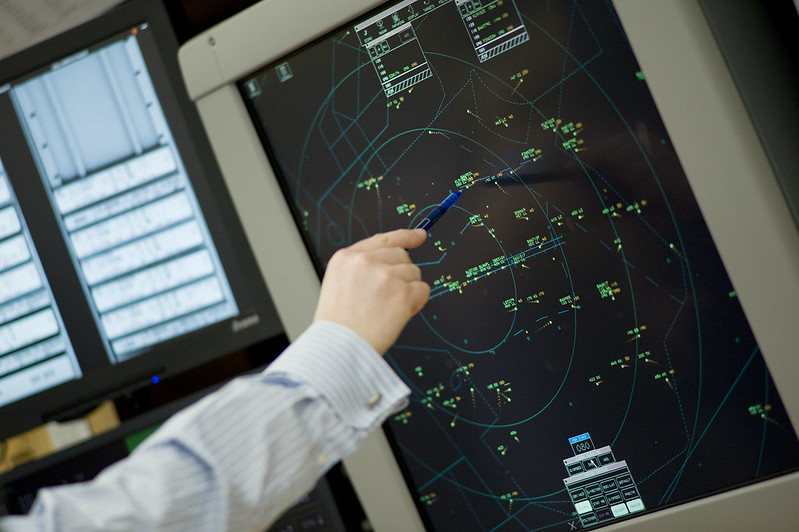
\includegraphics[width=0.85\textwidth]{pictures/nats_radar.jpg}
\caption{\label{fig:radar}A radar display at Swanwick \acrshort{atc} centre (\href{https://www.nats.aero/}{NATS}, \href{https://creativecommons.org/licenses/by-nc-nd/2.0/}{CC BY-NC-ND 2.0})}
\end{figure}

My project is an air traffic control simulator.
\acrfull{atc} is a service provided by air traffic controllers, who issue instructions and provide information to aircraft on the ground and in the air.
Air traffic controllers monitor the position of aircraft using radar, as shown in Figure \ref{fig:radar}, and communicate with pilots using radio\cite{caadef}.


\section{Analysis}
\subsection{Problem identification}
There are three main types of air traffic controllers: Aerodrome, Area, and Approach.

Aerodrome Controllers issue clearances to take off and land and route aircraft around the airfield; Area Controllers are responsible for aircraft in the climb, descent and en-route phases of flight; and Approach Controllers manage aircraft approaching an airport, putting them into the most efficient sequence to land\cite{natscareers}.

An air traffic controller is responsible for a particular section of \gls{airspace}.
Aircraft will arrive into their area of responsibility from certain points, and they will have to guide the traffic to the next controller's area of responsibility.
For example, a plane enters an approach control area descending from cruise, and the controller must guide them to an approach for a certain runway, where they are transferred to the aerodrome controller.

There are existing solutions for real-world training of air traffic controllers, and for public use.
Because the solutions for real-world controllers require certification, my solution will focus on public use.
My solution will aim to improve on the areas that are lacking in the existing publicly available solutions.

This problem is amenable to a computational approach because there is no other way to create this kind of simulation.
Real-world air traffic control relies heavily on computers.
This and the use of computational methods will be expanded on in the feature subsections of section \ref{essentialfeatures}.

\subsection{Stakeholders}
The two primary stakeholders for my solution are hobbyists and air traffic control organizations.
Their needs both include realism and ease of use.
The design section (\ref{design}) will discuss how decisions have been made to meet these needs.

\subsubsection{Air Traffic Control organizations}
The UK's \acrfull{nats} organization has a basic air traffic control game on their website for people to test their skills and determine if becoming an air traffic controller is right for them.
My solution could better solve that problem by providing a more realistic simulation, creating a more accurate test.
Other ATC organizations could promote the solution and make use of it to get people interested in air traffic control, making them more likely to take it up as a career, which is necessary as some \acrshort{atc} organizations struggle to recruit enough controllers\cite{indiaatcshortage}.

\subsubsection{Hobbyists}
Providing air traffic control is challenging and high-pressure.
It involves reacting to novel situations; thinking and planning ahead; and executing to move aeroplanes as safely and quickly as possible\cite{natsbuzz}.
For this reason, many people find it enjoyable to play the role of \acrshort{atc} in a simulator -- the \acrfull{vatsim}\footnote{\url{https://vatsim.net}} has over 100,000 active members as of 2023.
These users likely have an interest in air traffic control generally or want to become a controller in real life.
They will make use of the solution for entertainment as well as personal training in skills such as multitasking and problem-solving.
Because of their interests, they are likely to own a desktop or laptop computer.

Representing this group is Freddy.
He is a sixth form student who is interested in and knowledgeable about Air Traffic Control, wanting to become an RAF Air Traffic Controller in the future.
He has used multiple air traffic control simulators including Tower3D Pro and Endless ATC.
He can therefore provide very useful feedback on my solution.


\subsection{Existing solutions} \label{existingsolutions}
\subsubsection{ATC-SIM} \label{atc-sim}
\begin{figure}[H]
\centering
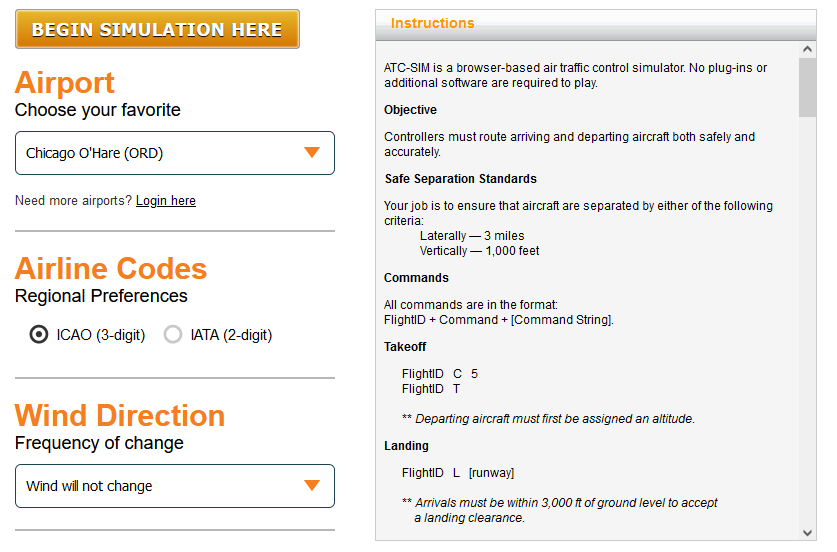
\includegraphics[width=0.7\textwidth]{existing_solutions/atcsimmenu.png}
\caption{\label{fig:atcsimmenu}ATC-SIM Main Menu}
\end{figure}
ATC-SIM\footnote{\url{https://atc-sim.com/}} is a browser-based air traffic control simulator which focuses on approach and tower control.
On the menu screen shown in Figure \ref{fig:atcsimmenu}, the user can select which airport they would like to control at and other preferences such as how much the wind will change.
It also shows instructions for the main part of the game.
The user can then press 'begin simulation here' to start, which takes them to the gameplay screen.
This serves its purpose well.
\begin{figure}[H]
\centering
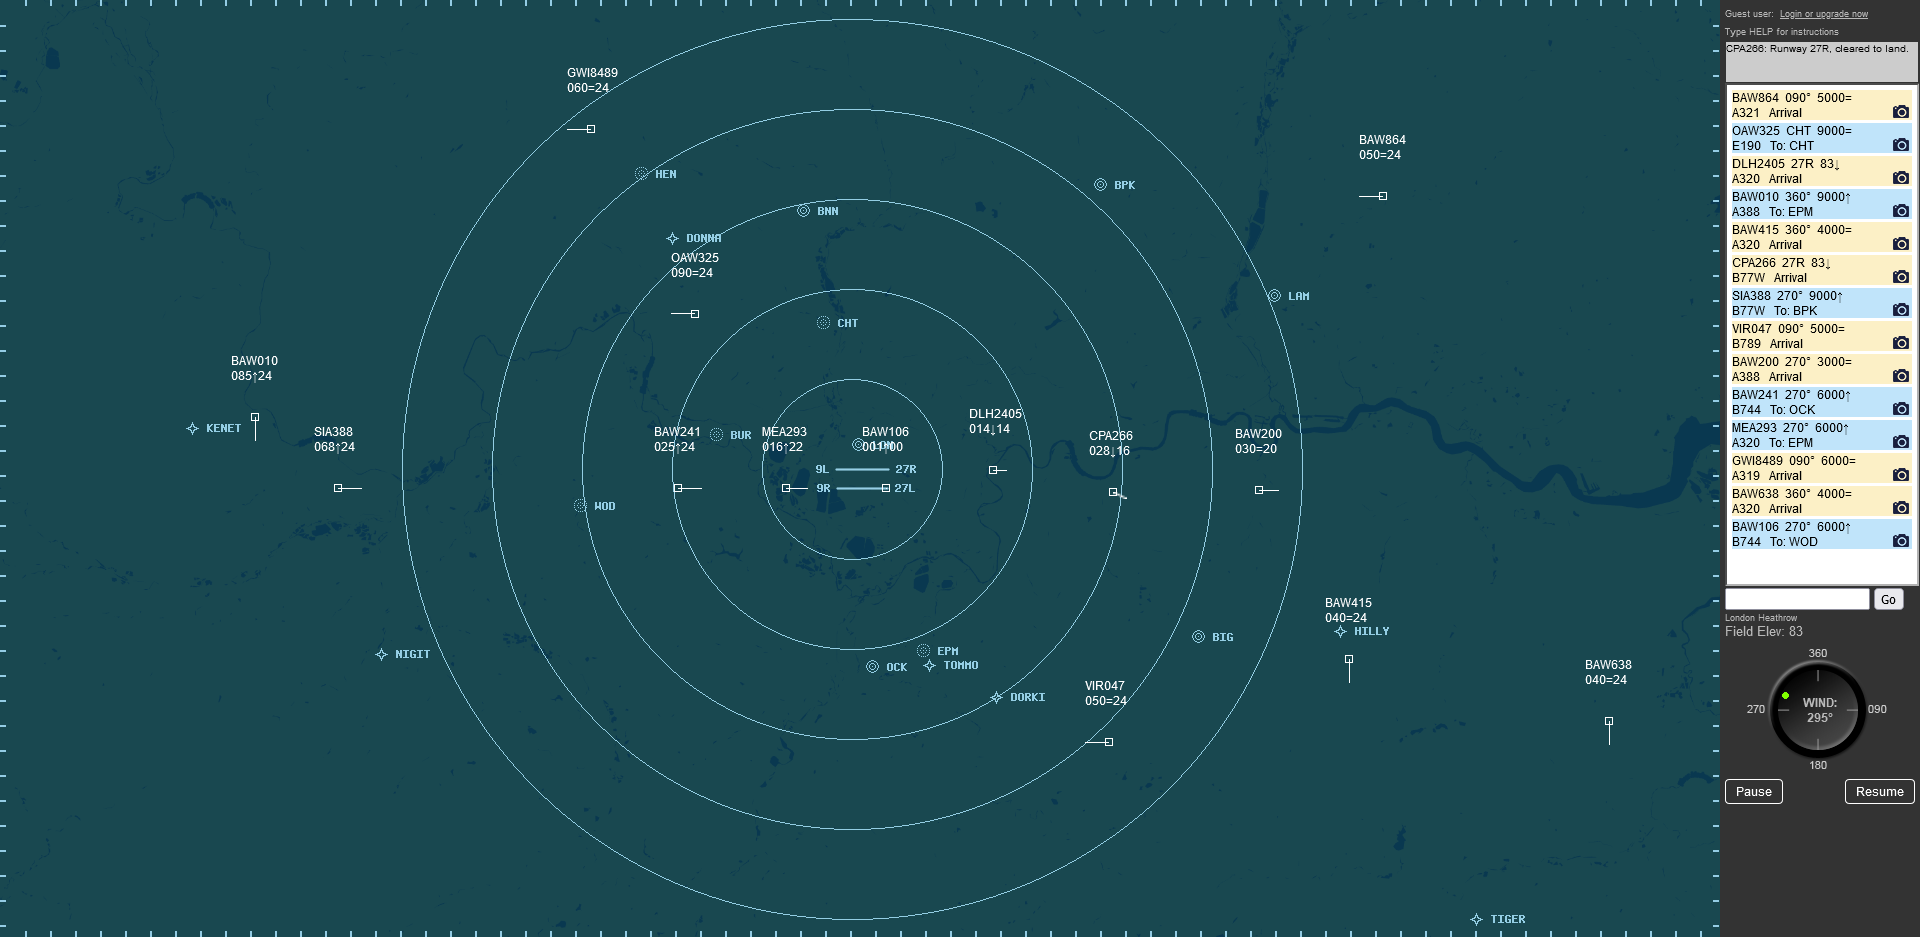
\includegraphics[width=0.85\textwidth]{existing_solutions/atcsim1.png}
\caption{\label{fig:atcsim1}ATC-SIM Gameplay Screen}
\end{figure}
The user can issue instructions to aeroplanes by entering abbreviated text commands into a text box, e.g. "BAW123 C 5" is an instruction for that aeroplane ("BAW123") to climb or descend to 5,000ft.
As seen in Figure \ref{fig:atcsim1}, a list of aeroplanes under the user's control is on the right-hand side of the screen.
On the central screen, text next to each aeroplane displays their current altitude, heading, and speed.
A display on the right-hand side shows the current wind speed and direction.
A background image shows the terrain and areas of water.

The view cannot be panned or zoomed and if the size of the browser window changes, the background moves but the waypoints don't, resulting in a visual mismatch (see Figure \ref{fig:airportinseaatcsim}).
Only a limited number of waypoints are available for the user to direct the aeroplane to.
There is no visual indication of the approach path, which makes it impossible for the user to accurately guide aeroplanes in.
Overall this is a reasonable solution for some but will disappoint more knowledgeable users.

\subsubsection{Endless ATC} \label{endlessatc}
\begin{figure}[H]
\centering
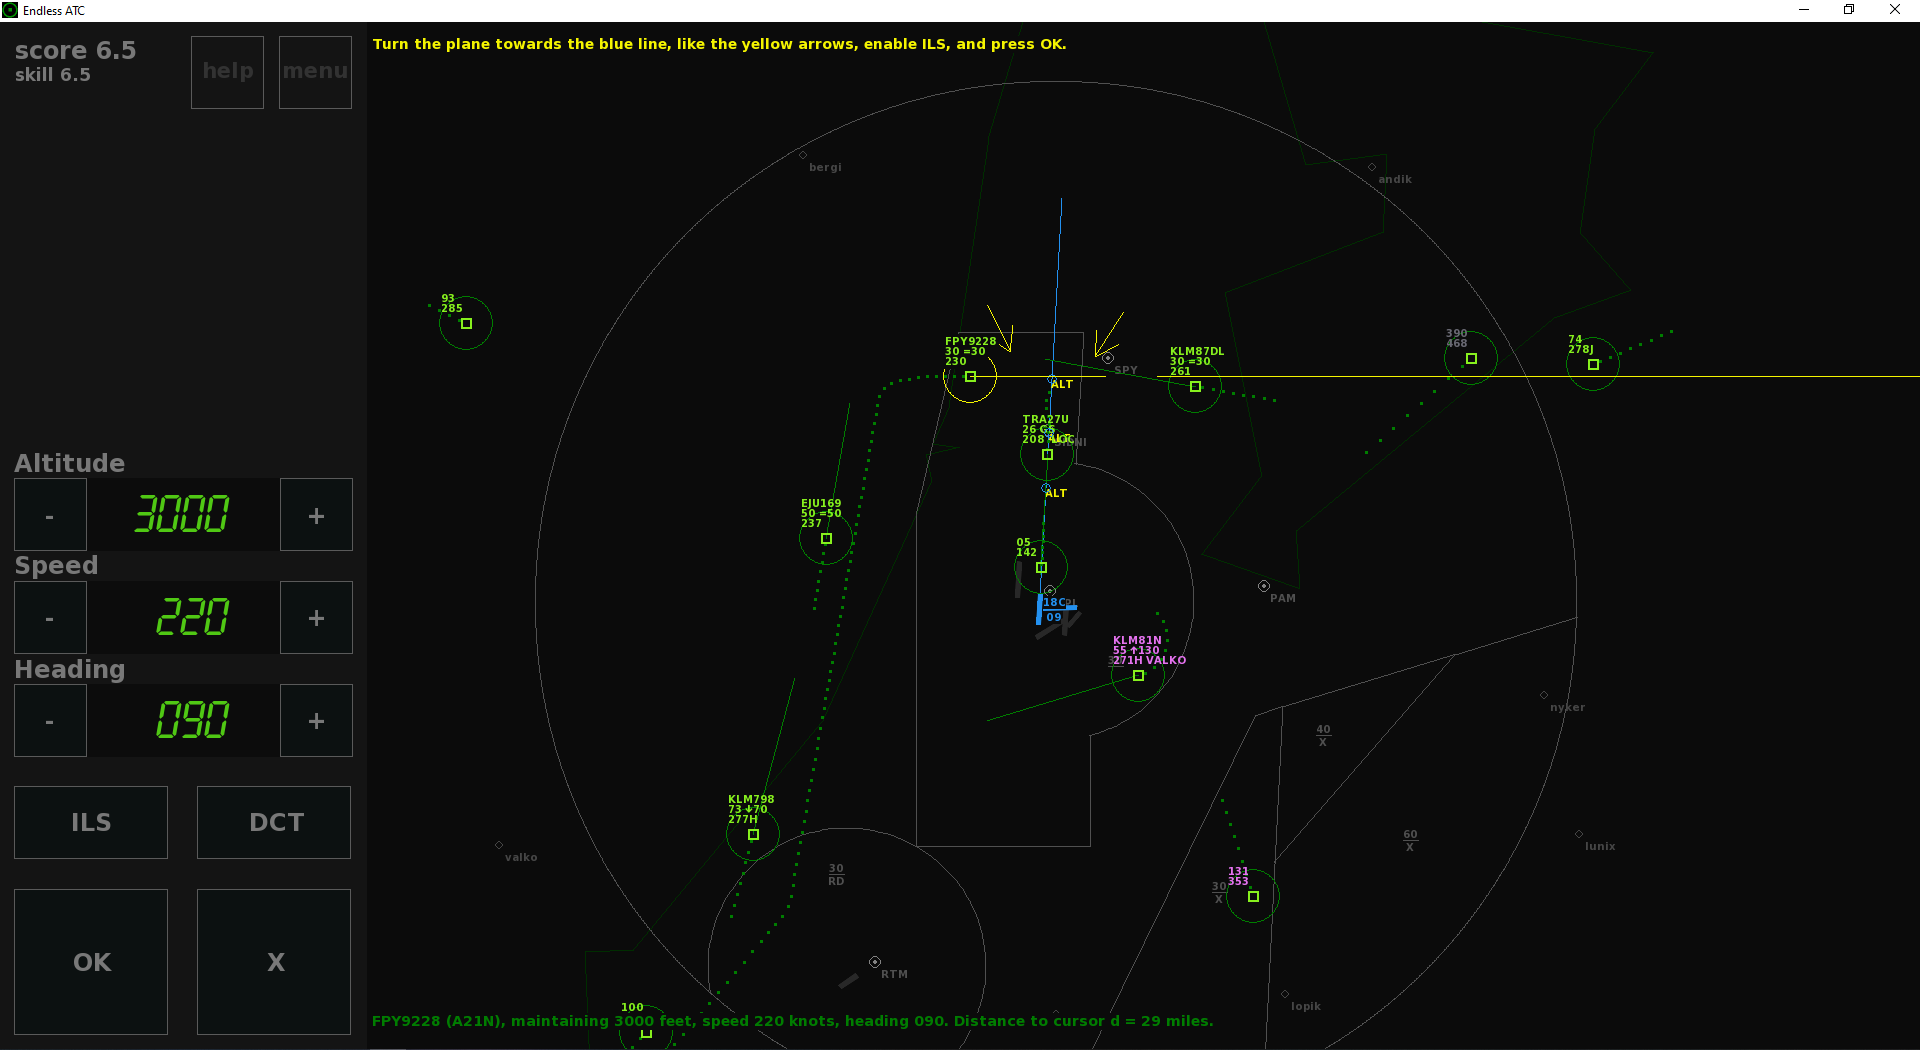
\includegraphics[width=0.85\textwidth]{existing_solutions/endlessatc.png}
\caption{\label{fig:endlessatc1}Endless ATC}
\end{figure}
Endless ATC\footnote{\url{https://startgrid.itch.io/endlessatc}} is a desktop and mobile air traffic control simulator focused on approach control.
The user can issue headings to aeroplanes by clicking or tapping on them and then moving their cursor in the direction of the desired heading.
The view can be panned around with the mouse and zoomed in with the scroll wheel.
Buttons on the side allow the user to change altitude, speed, and heading, or they can use various keys such as the scroll wheel to quickly change these values.

Once values have been changed, a button must be pressed to confirm or cancel the instructions.
A problem is that an instruction is also confirmed when the user clicks away or onto another aeroplane, potentially leading to confirming an instruction the user didn't mean to.
Text next to each aeroplane displays their current altitude, heading, and speed.
A limited number of waypoints are available which aeroplanes can be directed to by clicking and dragging to them.
The coastline is shown with overly simple lines.
A limited number of customization options are available, such as changing the aeroplane icons.
Another issue is that the user can only give altitude instructions in increments of thousands of feet, whereas it is very common in reality for controllers to give instructions involving hundreds of feet.


\subsection{Features} \label{essentialfeatures}
\subsubsection{Simulated aeroplanes}
The aim of my solution is to simulate the role of an air traffic controller, and the user will therefore need some traffic to control.
Whilst some solutions require other people to 'fly' the aeroplanes, mine should allow someone to use the simulation without any additional people, making it more flexible.
To achieve this the air traffic will have to be simulated by a computer.
This will involve repeatedly calculating the aeroplane's movement many times a second based on their speed and direction, and other factors such as wind.
This can be achieved with an algorithm and mathematical calculations which are suited to being run on a computer, allowing many aeroplanes to be simulated concurrently.

These aeroplanes will be abstracted from reality, only simulating the variables that are necessary to appear realistic on a radar screen.
For example, lift does not have to be simulated --- instead it can just be stated that the aeroplane is at a particular altitude.
To make them behave realistically however, it is necessary to simulate abstractions of e.g.
the pitch of the aeroplane, because this affects how long it takes for the aeroplane to change altitude.
Because the pitch required to maintain a certain \gls{flightpathangle} changes dependent on factors that would be complicated to simulate, such as lift and speed, I can instead model vertical motion only by the \gls{flightpathangle} (see figure \ref{fig:pitchfpa}), which allows for the same realistic behaviour without having to calculate the pitch.

\begin{figure}[H]
\centering
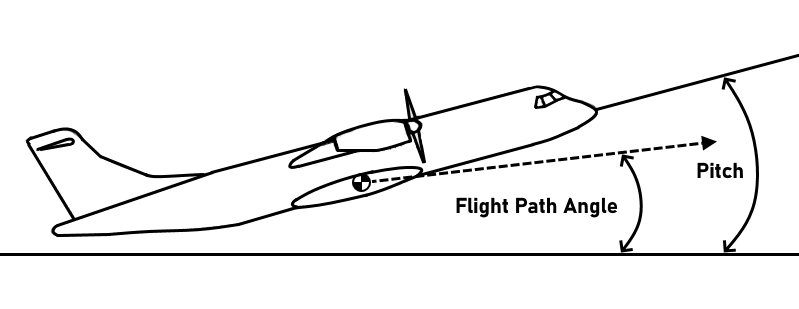
\includegraphics[width=0.7\textwidth]{diagrams/pitchfpa.png}
\caption{\label{fig:pitchfpa}Pitch and FPA}
\end{figure}

A simulation of the takeoff procedures of the aeroplane, such as its acceleration on the ground and initial rotation, will not need to be included because the solution is focussed on approach control.
Aeroplanes landing can also be largely simplified because below a certain altitude they will not be visible on the radar anyway.

Controllers often direct aeroplanes by telling them to fly on a certain heading.
The heading of an aeroplane describes the direction it is pointing in which, because of wind, is not necessarily the same as the direction it is travelling in (see Figure \ref{fig:windtriangle}).
Therefore controllers have to account for this when giving headings so that the aeroplane's actual track is in the intended direction.
This is a big part of the controller's job, so it will be necessary to simulate this.
The input to this will be a wind direction and a wind speed, live data for which could be obtained from an internet API.

\begin{figure}[H]
\centering
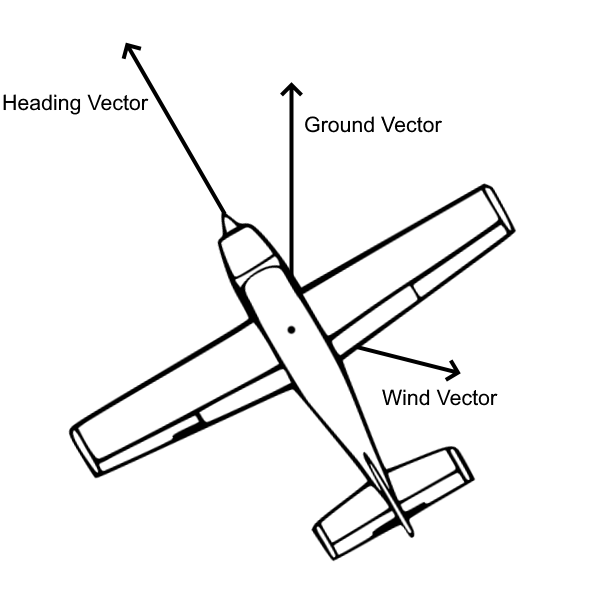
\includegraphics[width=0.5\textwidth]{diagrams/windtriangle.png}
\caption{\label{fig:windtriangle}The wind triangle}
\end{figure}

In addition to the base physics simulation, the aeroplanes will have simulated guidance systems so that they can follow the instructions defined in section \ref{aeroplaneinstructions}, one of the more complex being to follow an instrument landing system path to a landing.
An instrument landing system uses radio beacons to guide the aircraft laterally (with the localizer) and vertically (the glideslope) to a landing on the runway it is configured at, as shown in figure \ref{fig:ils}.
This can also be abstracted by not simulating the radio signals themselves.

\begin{figure}[H]
\centering
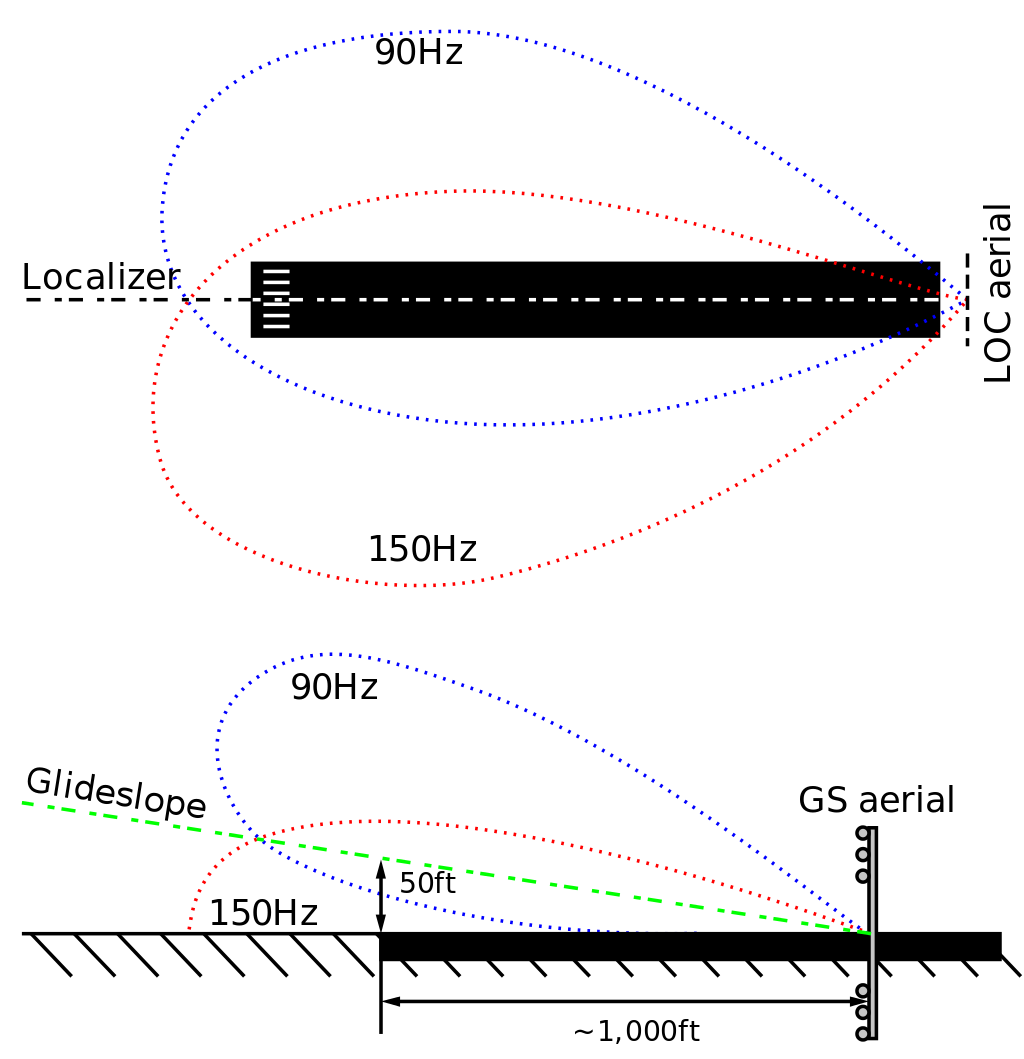
\includegraphics[width=0.5\textwidth]{context/ils.png}
\caption{\label{fig:ils}\acrfull{ils} (\href{https://commons.wikimedia.org/wiki/User:Fred_the_Oyster}{Fred the Oyster}, \href{https://creativecommons.org/licenses/by-sa/4.0/deed.en}{CC BY-SA 4.0})}
\end{figure}

\paragraph{Success criteria}
\begin{itemize}
    \item The aeroplane should be able to guide itself realistically in following instructions, including on an \acrshort{ils} (\ref{aeroplaneinstructions})
    \item The aeroplane should take a realistic amount of time to change altitude and heading
    \item Timescales should always be accurate, independent of the performance of the simulation
    \item The aeroplane's course should be accurately affected by wind
    \item Fifteen or more aeroplanes should be able to be simulated simultaneously while maintaining performance, as this is how many a controller is typically required to control in real life
\end{itemize}

\subsubsection{Aeroplane instructions} \label{aeroplaneinstructions}
In reality, air traffic controllers instruct aeroplane pilots verbally over radio.
The aeroplanes in my solution will be simulated, so there will be no pilot to hear and parse an audio instruction.
Therefore an alternative method of giving these aeroplanes instructions will be needed.
The essential instructions necessary to guide an aeroplane to a landing are for it to fly on a \gls{heading} or to a \gls{waypoint}, change altitude or \gls{airspeed}, and perform an \gls{instrumentapproach}.

The solution will create an abstraction of the verbal instructions which hides some detail, for example the user could type a number into the corresponding box and the plane will decide whether it needs to climb or descend if its current altitude is above or below the entered value.
To parse the user's input, the program will need to make multiple decisions.
For example, if the first character of the input to the heading field is an 'L' it would follow the process for instructing a turn to the left.
Also if the text was the name of a waypoint, it would send an instruction to go direct to that waypoint rather than a heading instruction.

\paragraph{Success criteria}
\begin{itemize}
    \item The user should be able to give an instruction for an aircraft to fly on a \gls{heading} or to a \gls{waypoint}, change altitude or \gls{airspeed}, and perform an \gls{instrumentapproach}; and it should respond accordingly
    \item This system should function concurrently with the simulation of the aeroplane, so that it does not pause the aeroplane's movement
    \item The solution should allow the user to give instructions as quickly or quicker than they would be able to verbally in real life
    \item To make the experience more fluid, it should also require as few button presses or mouse clicks as possible
\end{itemize}

\subsubsection{Displaying aeroplanes}
A representation of the aeroplane will need to be shown.
It will need to show their assigned heading or waypoint, altitude, and speed; their current heading or targeted waypoint, altitude, and speed; and their callsign.
As with real life radar displays, it should show a trail of dots or other symbols behind the aeroplane to illustrate its path and a line in front to show its current direction of travel.
It should be visually similar to real life for additional realism, including mimicking how quickly the display properties update, e.g. the radar only completes a full sweep every 4 seconds.
This can only be accomplished with a computer because of its unique ability to render custom, moving and changing graphics to display on an output device such as a monitor.

\paragraph{Success criteria}
\begin{itemize}
    \item The assigned heading or waypoint, altitude, and speed; current heading or targeted waypoint, altitude, speed, and callsign should be displayed
    \item Properties should update at a realistic rate: position every 4 seconds, and others at around every 0.5 seconds
    \item Every time the position updates, a history dot should be created up to a specified number, and they should then follow behind
\end{itemize}

\subsubsection{Traffic Simulation}
Once an aeroplane can be simulated, the creation of them must be controlled.
In the real world, the number of aeroplanes entering the controller's area of responsibility and departing changes based on airline timetables.
This data is unavailable, so an approximation can be used.
Aeroplanes will enter and exit the controller's area of responsibility via certain waypoints.

\paragraph{Success criteria}
\begin{itemize}
    \item Aeroplanes should enter the user's area of responsibility periodically from certain waypoints
    \item Aeroplanes should appear on the screen after taking off from a runway periodically
\end{itemize}

\subsubsection{Waypoints}
\begin{figure}[H]
\centering
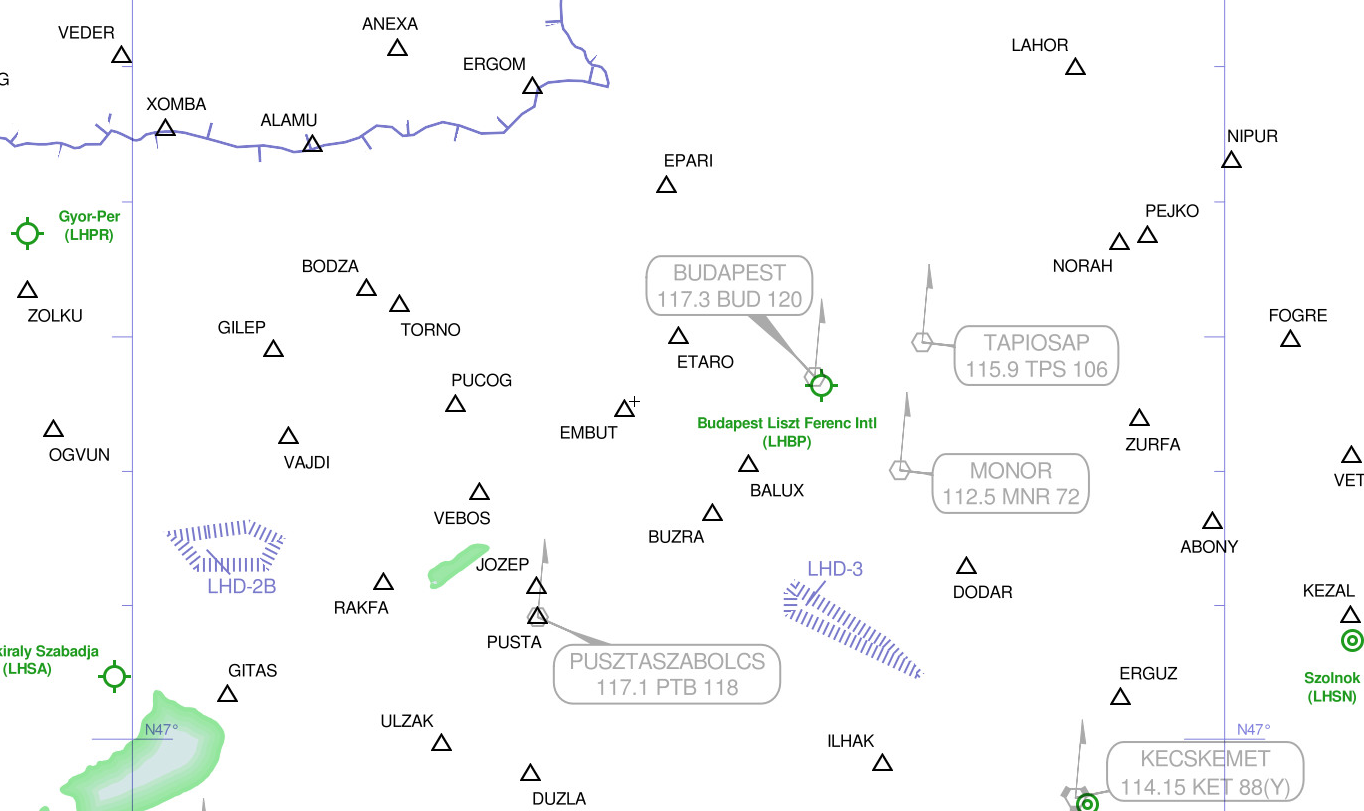
\includegraphics[width=0.7\textwidth]{context/budapest.png}
\caption{\label{fig:budapest}Map showing waypoints around Budapest International Airport}
\end{figure}

Waypoints are points, defined by latitude and longitude and given five-letter names, which are used for air navigation.
They are created specifically for that purpose and usually have no connection to features of the real world\cite{waypoint}.
A commercial airliner's route from one airport to another --- its flight plan --- is largely defined as a series of waypoints which it will fly between.
Air traffic controllers often take advantage of waypoints to direct traffic, instructing them to 'fly direct' to a named waypoint, for example "BAW123, route direct WILLO".

Waypoints are indispensable to air traffic controllers, therefore it is necessary to include them in my solution.
This will require data to be sourced with the names and GPS coordinates of the waypoints.
The waypoints should be shown on the screen in the correct position with a symbol corresponding to their type, and their name.

\paragraph{Success criteria}
\begin{itemize}
    \item Waypoints should appear in the correct position on the screen
    \item Their name should be shown next to an icon which changes based on the type of waypoint
    \item As many as 30 or more waypoints should be able to be displayed at once, since this is how many are present around some airports
\end{itemize}

\subsubsection{Pan and Zoom}
The user should be able to pan and zoom their view of the simulated radar screen.
This way they can more clearly see important areas where the majority of traffic is concentrated, rather than being limited to a fixed view.
This is especially useful where the approach control airspace area is very large and it otherwise would not be possible to simulate because there would not be enough room on the screen.
Being able to pan and zoom is also a feature of most modern real world radar screens.
To make interacting with the solution as enjoyable as possible and as professional as the real world equivalents, panning and zooming should be smooth; at a fixed speed and in fixed steps; and the camera should zoom towards the centre of the screen.
This will also create a familiar experience which is intuitive.

\paragraph{Success criteria}
\begin{itemize}
    \item Panning and zooming should be smooth
    \item It should occur at a fixed speed and in fixed steps
    \item The camera should zoom towards the centre of the screen
\end{itemize}

\subsubsection{Geographical features}
To make the simulated radar screen look realistic, it should be able to draw some kind of representation of the terrain.
Like in Endless ATC (\ref{endlessatc}), this can be a line showing the local coastline.
This is important because controllers should know if an aircraft is over water.
A large amount of data will need to be sourced representing this, which will then have to be processed and displayed.
This is a task very suited to being run a computer because of the storage and intensive processing of data.
This data will ultimately be represented using many latitude and longitude points, and looping will be necessary to apply processing to all of them.

\paragraph{Success criteria}
\begin{itemize}
    \item An abstraction of the terrain should be displayed
    \item It should appear accurate, having the correct proportions and with no breaks in lines
    \item It should respect the current scale of the display
\end{itemize}

\subsubsection{Extended centrelines}
\begin{figure}[H]
\centering
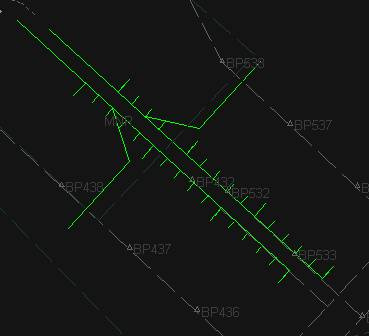
\includegraphics[width=0.6\textwidth]{context/centrelines.jpg}
\caption{\label{fig:centrelines}Extended centrelines in another solution}
\end{figure}
For every instrument approach (\acrshort{ils}) available at the airport the user is controlling at, a line extending from the threshold of the relevant runway in the direction of the localizer should be displayed and distance markers should be shown along it (like in figure \ref{fig:centrelines}).
As in real life, this feature is vital for the user to be able to direct aeroplanes to the instrument approach correctly, for which they need to see exactly where it is.
The distance markers are also important so that the controller can maintain a safe separation between aeroplanes.
This feature would make a big improvement over ATC-Sim (section \ref{atc-sim}).

\paragraph{Success criteria}
\begin{itemize}
    \item The line should be in the correct position and direction
    \item Distance markings should be shown at the correct intervals
\end{itemize}


\clearpage
\subsection{Limitations}
A few limitations must be stated to prevent the solution from becoming overly complex and to limit the scope.
They are as follows:
\begin{itemize}
    \item The simulator will only load information such as waypoints and terrain in a small area around the airport --- it will not allow the user to pan around the whole world at once.
    Doing so would require streaming the data in as the user moved around, which would be unnecessarily complex to implement because the user is only controlling aeroplanes in one geographical area at a time anyway.
    \item The simulator will only simulate traffic under \acrfull{ifr}\footnote{\url{https://en.wikipedia.org/wiki/Instrument_flight_rules}} because their behaviour is predictable.
    Aeroplanes under \acrfull{vfr} are flown by the pilot with reference to visual landmarks which are not simulated.
    This is a fairly major limitation because at some airports \acrshort{vfr} traffic is very common, however the existing solutions researched also have this limitation.
    \item Different types of aircraft, e.g. helicopters, will not be simulated because the way they behave is very different to fixed-wing aircraft and in most airports it is not common to see them.
    The manoeuvring characteristics used will be an approximation of an average airliner, rather than having different data for different types.
    \item \Gls{airspace} boundaries will not be simulated because it is too difficult to obtain the data defining them; and even if it could be sourced, it would also be difficult to calculate whether an aircraft was within a certain area of airspace because their areas are defined by a series of points.
    It is also not very necessary because at most airports there is a large open area of \gls{airspace}, so considering it does not enter into the workload of the controller much; so excluding it would not decrease realism much.
\end{itemize}


% \subsection{Success criteria}


\subsection{Requirements}
In order to make the solution accessible to as many people as possible, the program should not require any additional software to be downloaded to the user's device for it to function.
However there are two problems that mean my solution will be limited to a desktop or laptop computer.
Firstly, the complex inputs necessary for directing air traffic, which rules out devices without the facilities for a keyboard and mouse such as consoles.
Secondly, the large area of information which has to be displayed, which rules out devices with small screens such as smartphones.
However this will not present an issue, because the majority of stakeholders in the solution will have a computer.

To the same end, it should function well on a computer with very minimal specifications, for instance a 2GHz dual-core processor with integrated graphics, 4 GB of RAM, and a 120 GB hard drive.
The program should function on Windows, Linux, and macOS systems.
\clearpage

\begin{sidewaysfigure}
    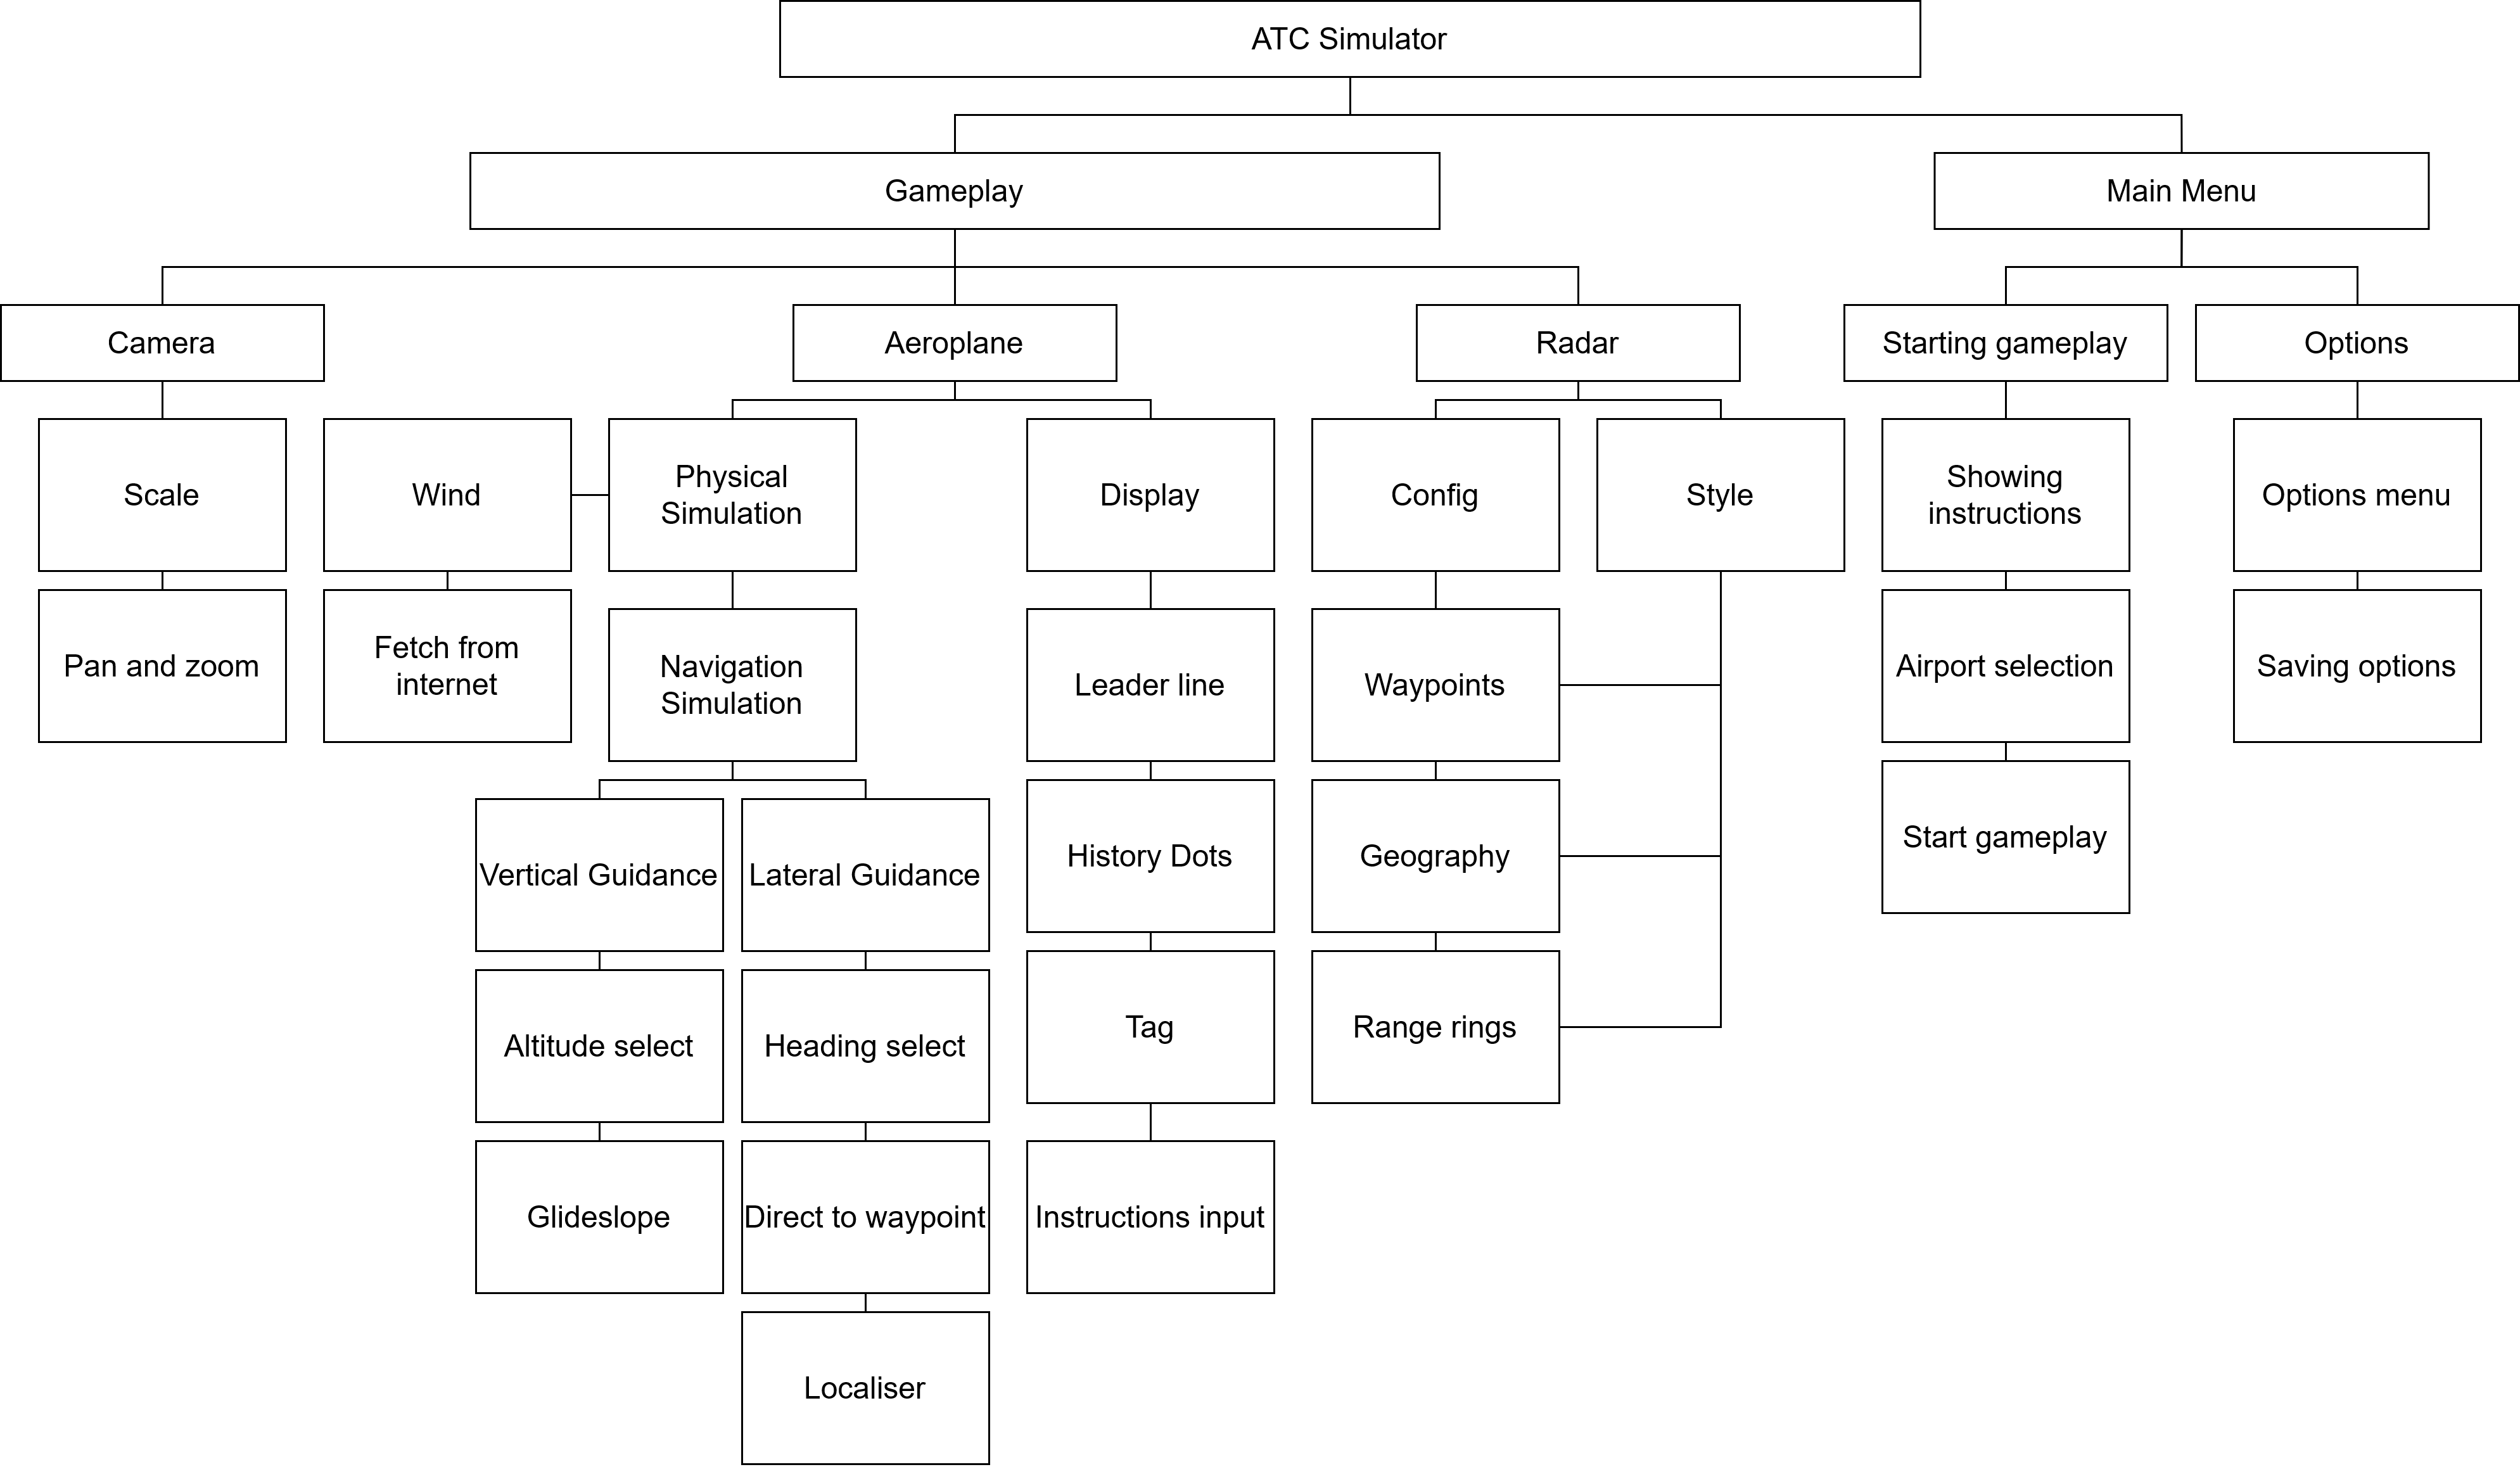
\includegraphics[width=\textwidth]{diagrams/problemdiagram.png}
    \caption{\label{fig:solution_diagram}Solution diagram}
\end{sidewaysfigure}

\clearpage

\section{Design} \label{design}
\subsection{Breakdown of the problem}
Figure \ref{fig:solution_diagram} shows how the problem has been broken down into smaller problems and sub-problems.
Breaking the problem down like this allows each to be solved independently, separating concerns and making development easier because changes to one area do not affect other areas.
The subsequent subsections and their organization will illustrate further the process of choosing how to break down the problem.


\subsection{Representing space}
My simulation will be simulating real-world places: airports and the world around them.
Therefore I cannot use arbitrary units for position or approximate where things are.
Equally, I cannot simulate motion or calculate where points of interest should appear on the screen using latitude and longitude values alone.
Therefore a working value of the lateral and vertical distances in nautical miles from a reference point must be used, which is calculated once using the latitudes and longitudes.
This abstraction removes the curvature of the earth.

\subsubsection{Scale}
That gives everything a position in nautical miles, which then needs to be converted to a number of pixels for it to be displayed.
A scale factor can be calculated by dividing the number of pixels available on the screen by the number of nautical miles that should be shown in that area.
The values in nautical miles can then simply be multiplied by this factor.

\subsubsection{Pan and zoom}
The initial scale can be calculated from a desired width in nautical miles specific to each airport configuration.
From there the user should be able to zoom in or out using the scroll wheel of their mouse.
Each time the user zooms in or out an increment, the scale value will be multiplied by e.g. 1.1 or 0.9 respectively.
Panning the simulated radar screen will be accomplished by recording the position of the user's mouse on the screen when they first press the right mouse button down, and then moving a virtual camera in the inverse direction to the motion of the mouse relative to that point.
This will be very usable for the user, because it is similar to other solutions.

\subsection{Simulated aeroplanes}
In order to maintain physical consistency (e.g. if an aeroplane is already in a turn to the right, it will take longer to start turning to the left than if it was not turning), the navigation system will be isolated from the physical simulation and will interact with it by commanding a yaw rate in degrees per second and a \gls{flightpathangle} in degrees.
I have chosen these parameters to provide a level of abstraction which is sufficiently realistic, while keeping complexity reasonably low.

\begin{figure}[H]
\centering
\begin{tabular}{ |l| } 
\hline
\multicolumn{1}{ |c| }{\textbf{Aeroplane}} \\
\hline
TrueAltitude : float \\
TrueAirspeed : float \\
TrueHeading : float \\
PositionNm : Vector2 \\
LateralGuidanceMode : LateralMode \\
VerticalGuidanceMode : VerticalMode \\
\hline
void PhysicsUpdate(float) \\
\hline
\end{tabular}
\caption{\label{fig:aeroplaneclass}Aeroplane class diagram}
\end{figure}

Figure \ref{fig:aeroplaneclass} shows the key attributes and methods of the aeroplane class which will be used.
Using a class enables many aeroplanes to be simulated at once, where each aeroplane is an instance of the class.
Keeping track of the many variables of each necessary for the physics and navigation simulation would otherwise be very difficult.
The attributes have been chosen because they are absolutely necessary for the simulation and a controller is concerned with them in real life.

\begin{figure}[H]
\centering
\begin{tabular}{ |c|c|c| }
\hline
Attribute & Units & Valid range \\
\hline
TrueAltitude & Feet & $x \geq 0$ \\
\hline
TrueAirspeed & Knots & $x \geq 0$ \\
\hline
TrueHeading & Degrees & $0 \leq x \leq 360$ \\
\hline
\end{tabular}
\caption{\label{fig:aeroplaneclassinputs}Aeroplane class input validation ranges}
\end{figure}

Figure \ref{fig:aeroplaneclassinputs} shows the valid ranges of the attributes of the Aeroplane class.
Attributes not shown in the table do not require validation because they do not receive user input.
TrueAltitude must be greater than zero because it represents height above terrain and the aeroplane should not go below it; TrueAirspeed cannot be less than zero because it represents forward speed through the air; and TrueHeading, being a heading, is by definition between zero and 360 degrees.
Ensuring that these values remain in a valid range means that all areas of the solution know what to expect and do not each have to do their own validation.

\subsubsection{Physics simulation}
\begin{figure}[H]
\centering
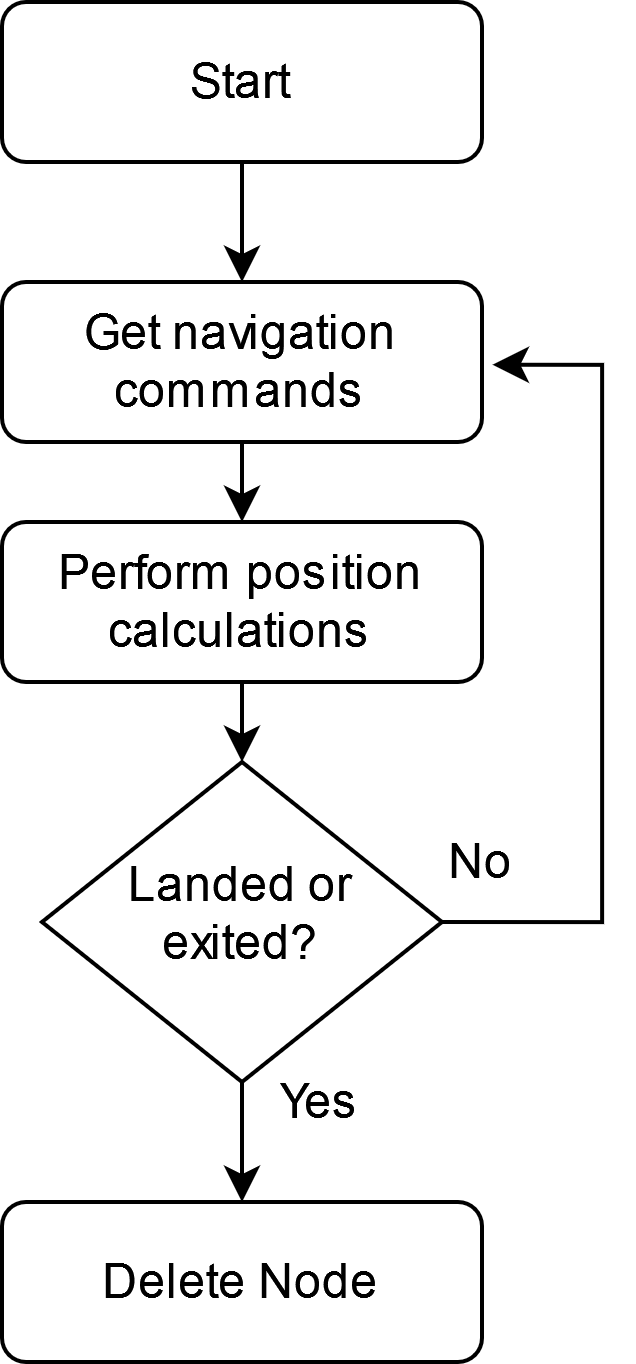
\includegraphics{diagrams/flowcharts/aeroplanesimulationprocess.png}
\caption{\label{fig:physics}Simulation loop}
\end{figure}

As shown in figure \ref{fig:physics}, the aeroplane physics simulation will use a loop in which it will talk to the navigation system to receive its commands for movement, and then update the flight parameters and re-calculate position.
In all calculations the real world time since the last loop iteration will be used to make sure that timescales, e.g. the time it takes for the aircraft to bank left and right, are consistent.
To simulate those times, the flight parameters will be moved towards the commanded values with a rate multiplied by the time delta on each iteration of the loop.
Through testing in a flight simulator I found typical values for those rates: yaw will change at a rate of $\frac{1}{2}$ degrees per second (per second); flight path angle at 0.17 degrees per second (per second); and airspeed at 1 knot per second.
These values will be stored in constant variables.
This loop should run many times a second to provide sufficient accuracy.

To perform the position update, the true heading of the aeroplane will be converted to a \gls{directionvector} which will be multiplied by the true airspeed.
The fact that the ground speed is lower given the same airspeed if the \gls{flightpathangle} deviates from zero will be accounted for using trigonometry.
Then the direction of the wind will be converted to a \gls{directionvector} which will be multiplied by the wind speed.
These vectors will then be added together to produce the ground vector.

\paragraph{Testing}
To test that the aeroplane responds correctly to wind, it should be tested with all different directions and plausible speeds of wind, while flying on different headings.
For example a 10 knot wind at a 90-degree angle to the aeroplane's heading should alter its course and increase its ground speed, but at an angle opposite to the aeroplane's heading it should only decrease its ground speed.

\subsubsection{Navigation simulation}
At all times, a separate lateral and vertical guidance mode will be engaged.
Making lateral and vertical modes independent of each other reduces code duplication because it is often required to have e.g. the same lateral behaviour with multiple vertical behaviours.
This also mirrors how autopilots work in reality.
Every simulation step, the active modes will be asked if they want to change to a different mode, which will be used for example when maintaining a heading while waiting to capture the localizer.
The modes will each be classes which will inherit from a parent class: LateralMode (figure \ref{fig:lateralmodeclass}) for the lateral modes and VerticalMode (figure \ref{fig:verticalmodeclass}) for the vertical modes, overriding e.g. the RollCommand method to implement their own functionality.
Because the LateralMode and VerticalMode classes have a common attribute of aeroplane, the aeroplane for which they are providing guidance, this will be in a parent class Mode with that attribute which they will inherit from.
Figure \ref{fig:vertnav} and \ref{fig:lnav} illustrate how the vertical and lateral guidance modes respectively of an aeroplane will change on certain conditions.
% The modes will each be classes which will implement \glspl{interface} stating that they include e.g. an update function.
\begin{figure}[H]
\centering
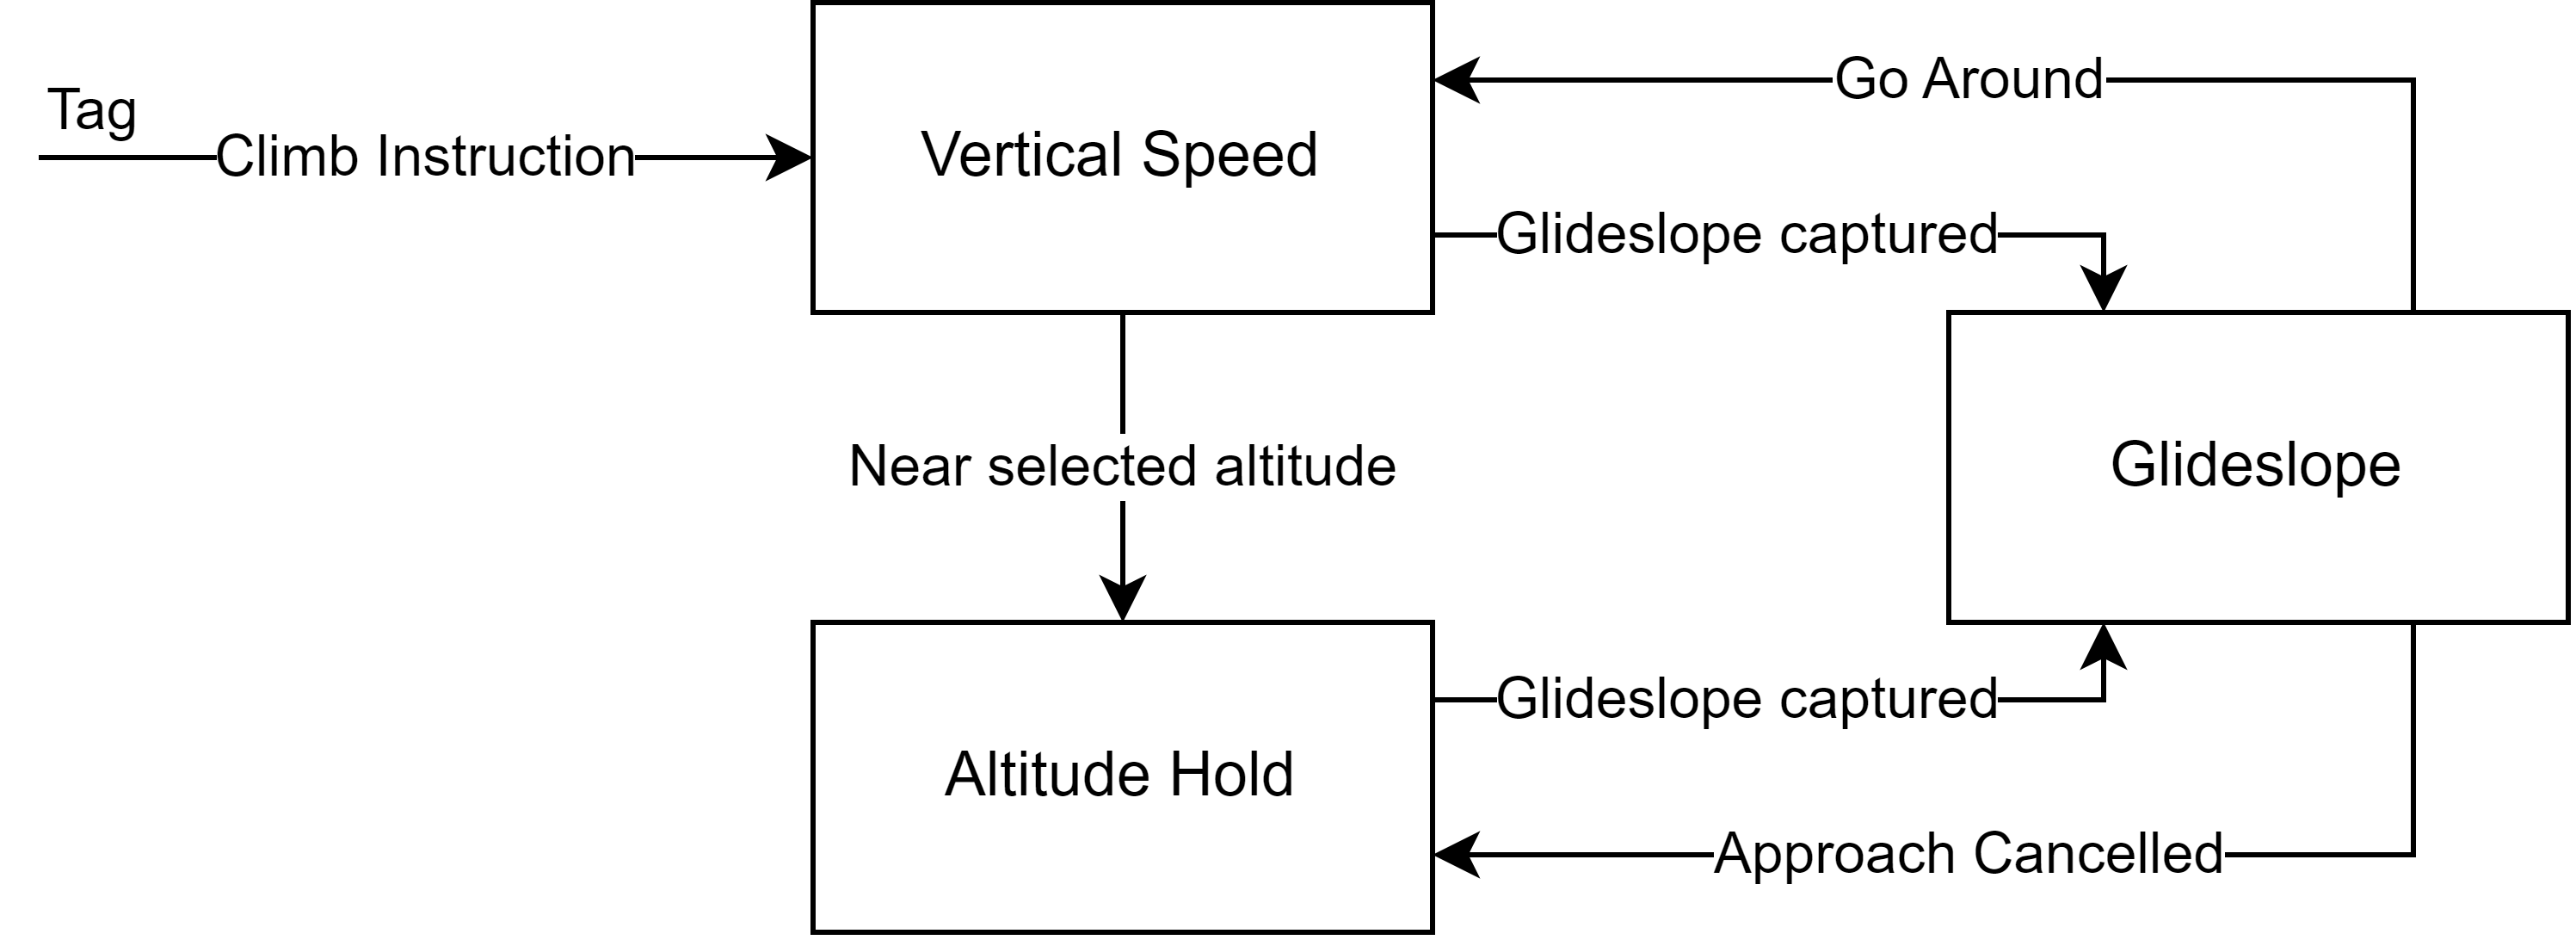
\includegraphics{diagrams/vertnav.png}
\caption{\label{fig:vertnav}State transitions between vertical guidance modes}
\end{figure}

\begin{figure}[H]
\centering
\begin{tabular}{ |l| } 
\hline
\multicolumn{1}{ |c| }{\textbf{VerticalMode : Mode}} \\
\hline
virtual float FlightPathAngleCommand() \\
virtual VerticalMode? NewMode() \\
\hline
\end{tabular}
\caption{\label{fig:verticalmodeclass}Vertical mode class diagram}
\end{figure}

\paragraph{Altitude change modes}
When an instruction to climb or descend is given a vertical guidance mode such as vertical speed will be engaged.
The vertical speed mode will control the commanded flight path angle to achieve the desired vertical speed, and then once the aeroplane is calculated to be close enough to the instructed altitude that if it levels off at the standard rate it will arrive at that altitude without over or undershooting, the mode will tell the guidance system to switch to the altitude hold mode.
Figure \ref{fig:verticalspeedmodeclass} shows the class which will implement the vertical speed mode, overriding the base FlightPathAngleCommand and NewMode methods and adding new attributes.
The class which implements the altitude hold mode does not override the base methods, which are to return zero for the FlightPathAngleCommand and null (i.e. do not change mode) for the NewMode method; it also does not require additional attributes.

\begin{figure}[H]
\centering
\begin{tabular}{ |l| } 
\hline
\multicolumn{1}{ |c| }{\textbf{VerticalSpeed : VerticalMode}} \\
\hline
float Altitude \\
float VerticalRate \\
\hline
override float FlightPathAngleCommand() \\
override VerticalMode? NewMode() \\
\hline
\end{tabular}
\caption{\label{fig:verticalspeedmodeclass}Vertical speed mode class diagram}
\end{figure}

\paragraph{Glideslope}
% When the aeroplane is cleared for an \acrshort{ils} approach, the active vertical guidance mode will wait until the aeroplane approaches an appropriate distance from the glideslope, and then tell the guidance system to switch to the glideslope follow mode which will command a pitch down to match the glideslope angle.
When the aeroplane is cleared for an \acrshort{ils} approach, the vertical guidance mode will be set to the glideslope mode (figure \ref{fig:glideslopemodeclass}).
It will use trigonometry calculate the current height of the glideslope beam at the aeroplane's position based on the position and elevation of the transmitter; and the angle of the glideslope (see figure \ref{fig:glideslope}).
It will subtract the aeroplane's height from the height of the glideslope to get the deviation from it in feet, and then use a PID Controller\footnote{\url{https://en.wikipedia.org/wiki/PID_controller}} to determine a flight path angle to correct on to the glideslope and follow it down.

\begin{figure}[H]
\centering
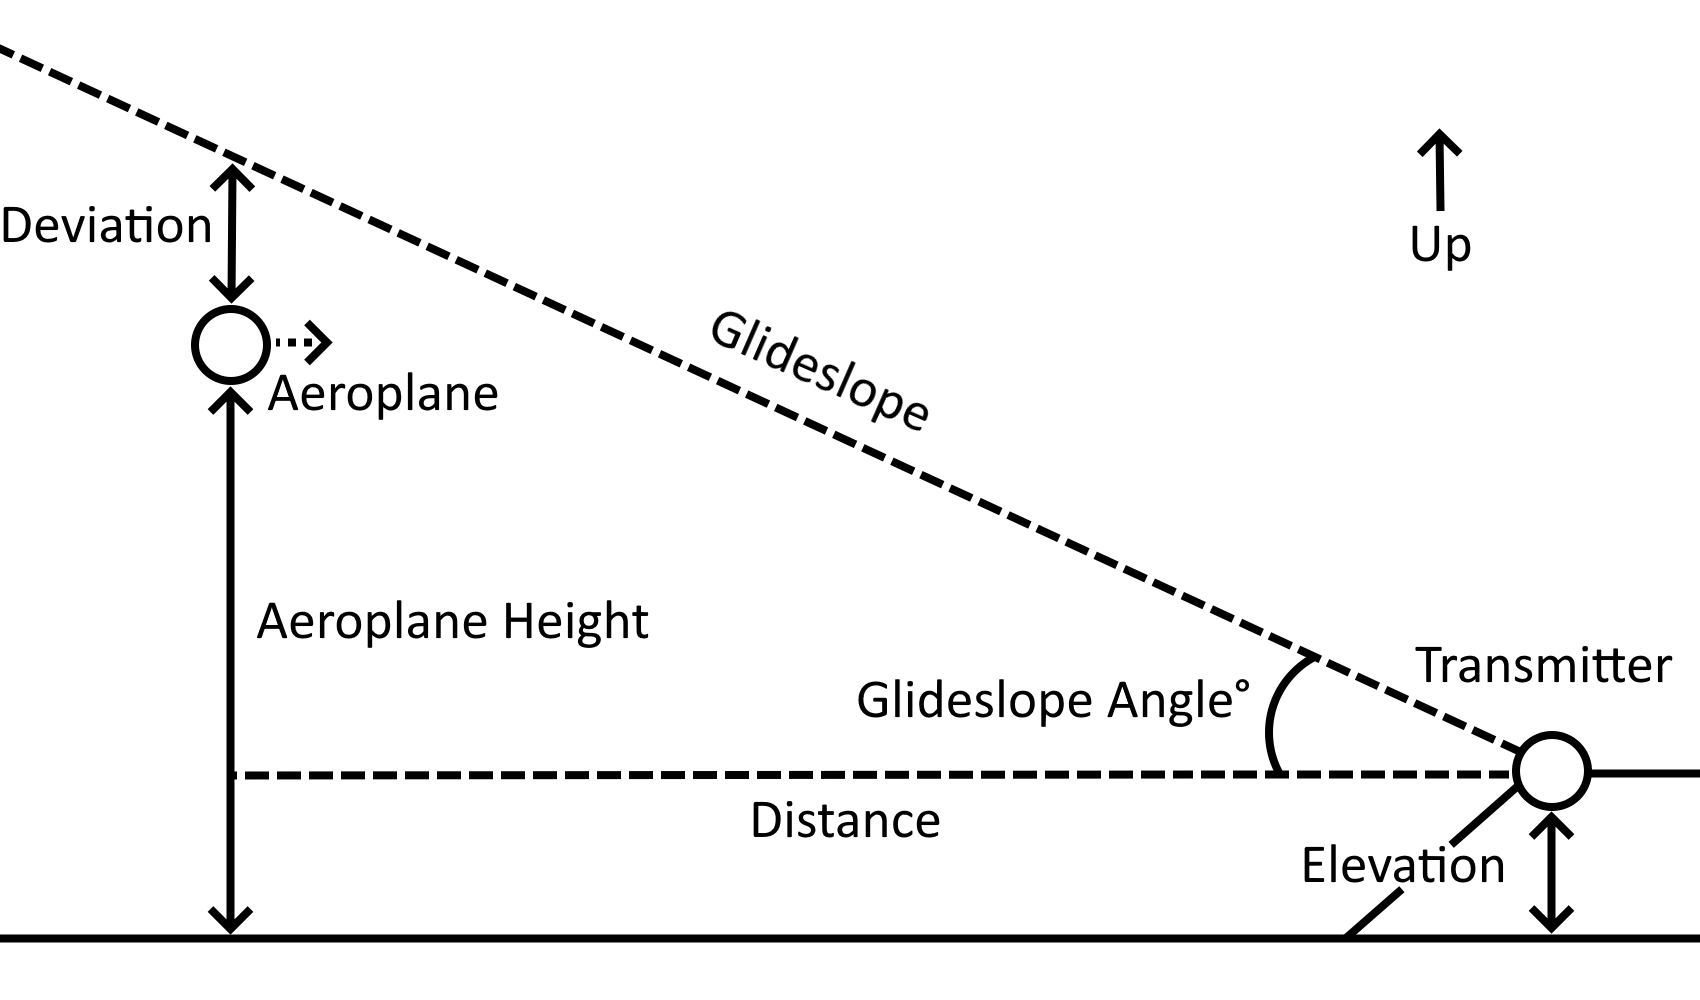
\includegraphics{diagrams/glideslope.png}
\caption{\label{fig:glideslope}Glideslope simulation diagram}
\end{figure}

\begin{figure}[H]
\centering
\begin{tabular}{ |l| } 
\hline
\multicolumn{1}{ |c| }{\textbf{Glideslope : VerticalMode}} \\
\hline
approach Approach \\
\hline
float Deviation() \\
override float FlightPathAngleCommand() \\
\hline
\end{tabular}
\caption{\label{fig:glideslopemodeclass}Glideslope mode class diagram}
\end{figure}

\begin{figure}[H]
\centering
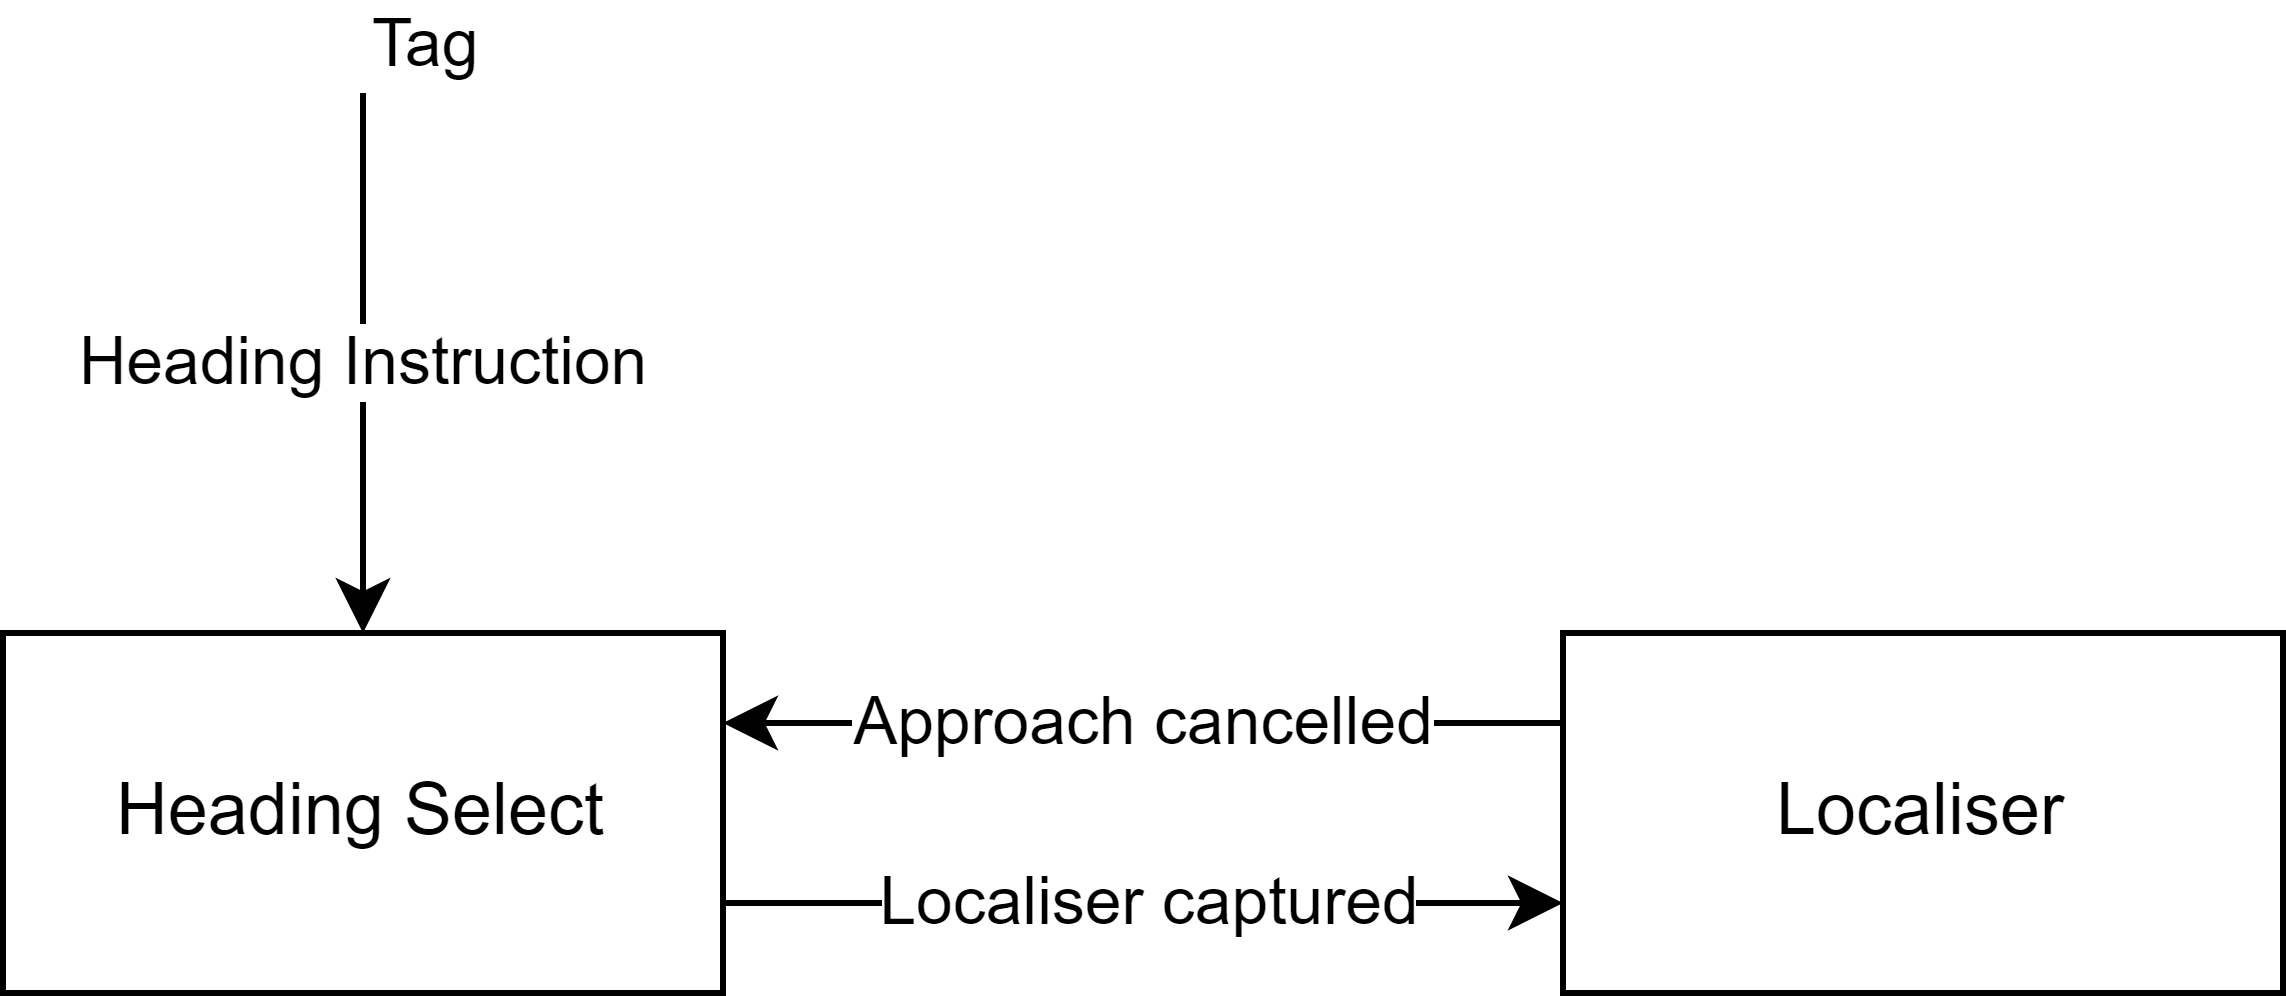
\includegraphics{diagrams/lnav.png}
\caption{\label{fig:lnav}State transitions between lateral modes}
\end{figure}

\begin{figure}[H]
\centering
\begin{tabular}{ |l| } 
\hline
\multicolumn{1}{ |c| }{\textbf{LateralMode : Mode}} \\
\hline
virtual float RollCommand() \\
virtual LateralMode? NewMode() \\
\hline
\end{tabular}
\caption{\label{fig:lateralmodeclass}Lateral mode class diagram}
\end{figure}

\paragraph{Heading select}
When receiving a heading instruction, the heading select lateral mode (figure \ref{fig:headingselectmodeclass}) will be set.
In addition to the heading to be followed, the instruction should include whether the aeroplane should turn in the quickest direction or a specific direction.
If the quickest direction is instructed, it will determine it by comparing the difference in degrees between the current and selected heading assuming a turn in each direction and see which is the smallest.
While the difference between the current and selected heading is less than that needed to roll out of the turn without overshooting, it will command the standard turn rate in the specified direction.

\begin{figure}[H]
\centering
\begin{tabular}{ |l| } 
\hline
\multicolumn{1}{ |c| }{\textbf{HeadingSelect : LateralMode}} \\
\hline
float selectedHeading \\
TurnDirection turnDirection \\
\hline
override float RollCommand() \\
\hline
\end{tabular}
\caption{\label{fig:headingselectmodeclass}Heading select mode class diagram}
\end{figure}

\paragraph{Localizer}
When the aeroplane is cleared for an \acrshort{ils} approach, the lateral guidance mode will be set to the localizer mode (figure \ref{fig:localizermodeclass}).
It will calculate the aeroplane's perpendicular distance (marked $x$ on figure \ref{fig:localizer}) from the localizer beam by calculating the bearing between the aeroplane's position and the localizer transmitter's position and comparing it with the \gls{heading} of the beam, then using trigonometry to calculate it from that angle.

\begin{figure}[H]
\centering
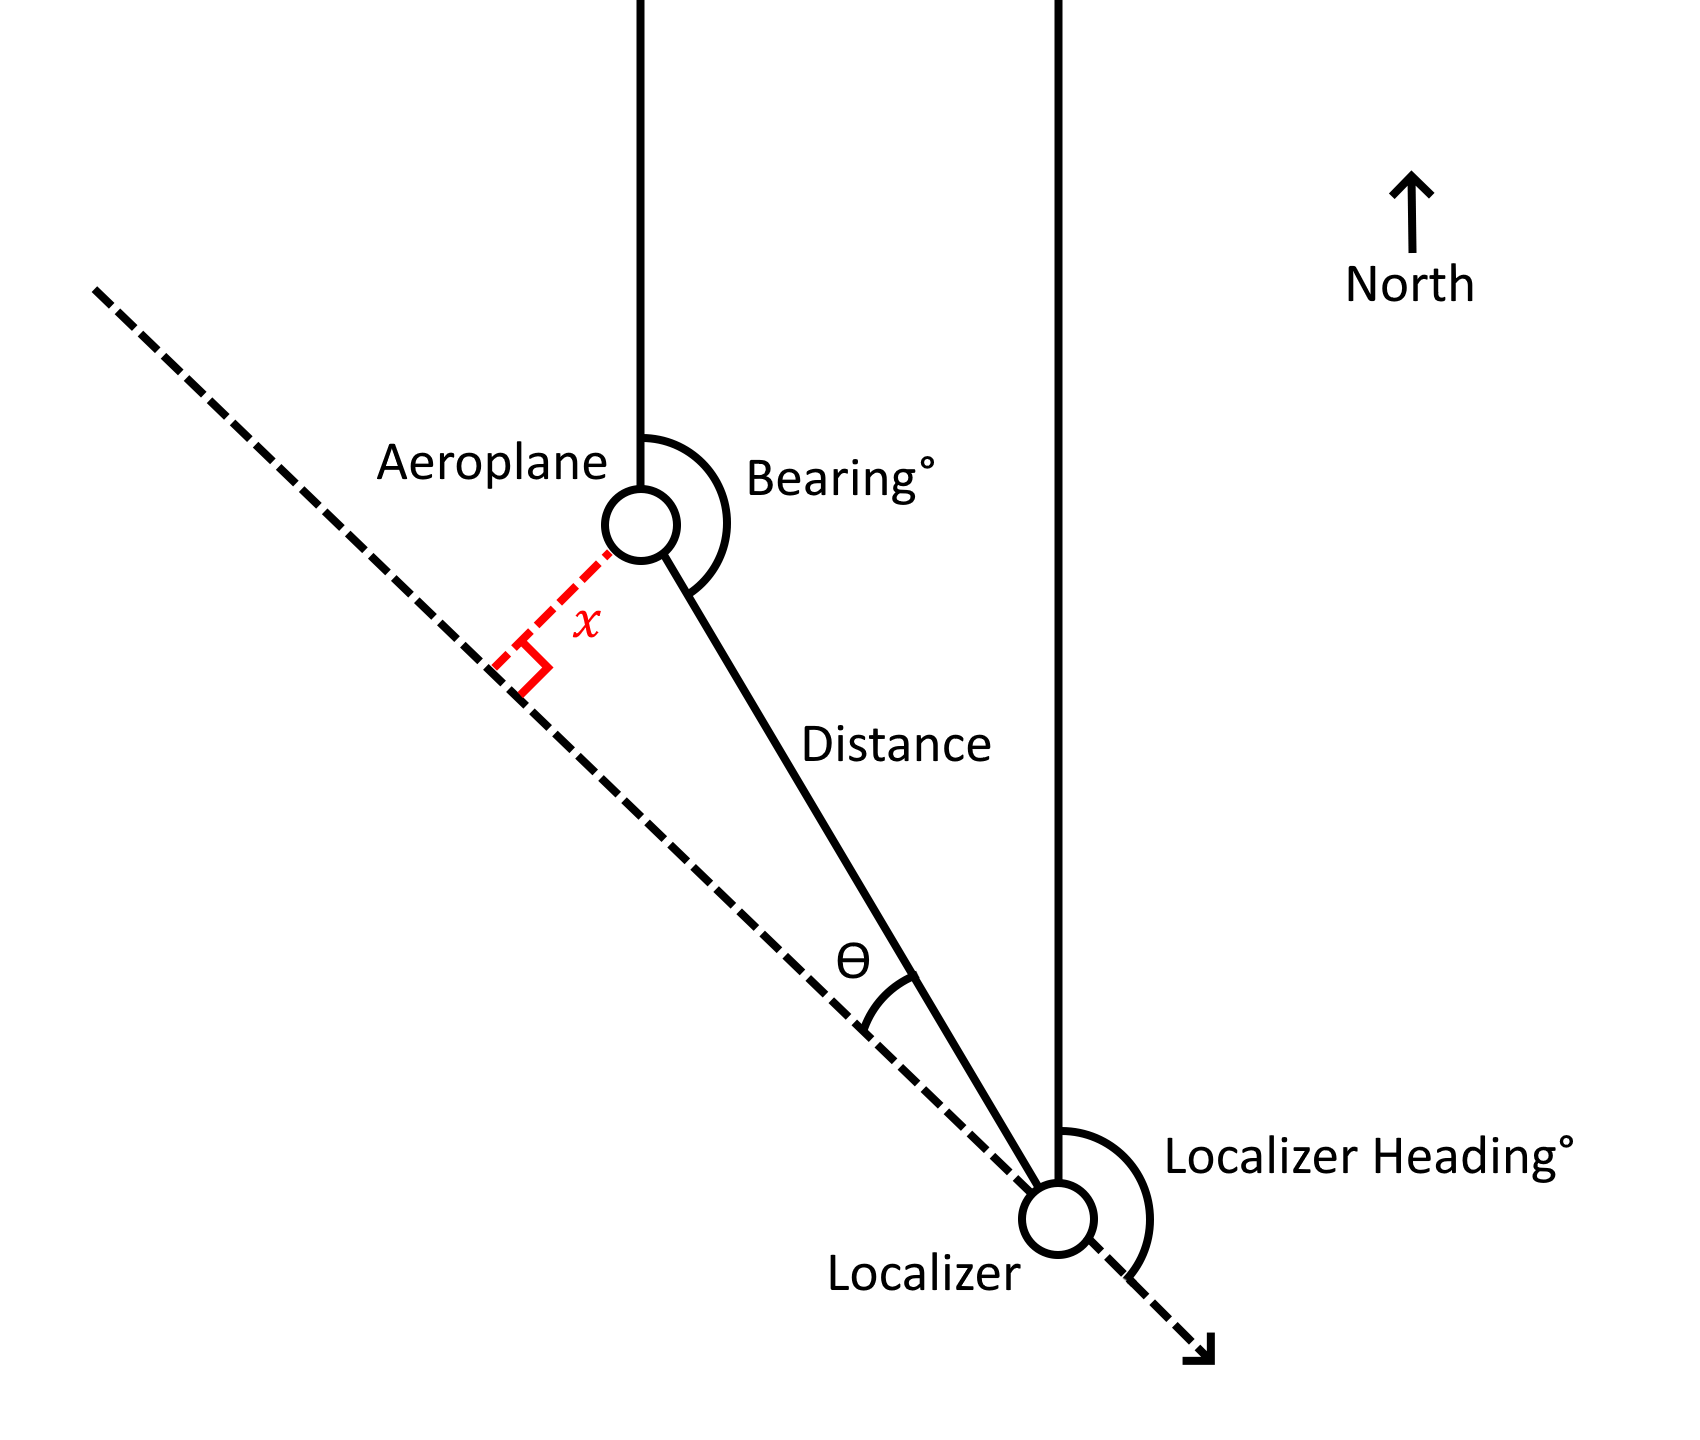
\includegraphics{diagrams/localizer.png}
\caption{\label{fig:localizer}Localizer simulation diagram}
\end{figure}

\begin{figure}[H]
\centering
\begin{tabular}{ |l| } 
\hline
\multicolumn{1}{ |c| }{\textbf{Localizer : LateralMode}} \\
\hline
approach Approach \\
\hline
float Deviation() \\
override float RollCommand() \\
\hline
\end{tabular}
\caption{\label{fig:localizermodeclass}Localizer mode class diagram}
\end{figure}

\paragraph{Direct to waypoint}
When receiving an instruction to fly direct to a waypoint, the direct lateral guidance mode (figure \ref{fig:directmodeclass}) will be set.
Because the aeroplane is affected by wind, the system must know the actual track over ground of the aeroplane so that it can travel in the direction of the selected waypoint, even though its commands to the physical simulation only directly affect heading.
To determine the track in degrees to target to fly towards the waypoint, the bearing must be calculated (see figure \ref{fig:directto}).
While the difference between the current and required track is less than that needed to roll out of the turn without overshooting, it will command the standard turn rate in the appropriate direction.
Once the distance to the selected waypoint is very small, the direct mode should tell the aeroplane to switch to a heading select mode maintaining the present heading.
Otherwise, the aeroplane would attempt to circle back around to the waypoint after flying over it which is not realistic or desired behaviour.

\begin{figure}[H]
\centering
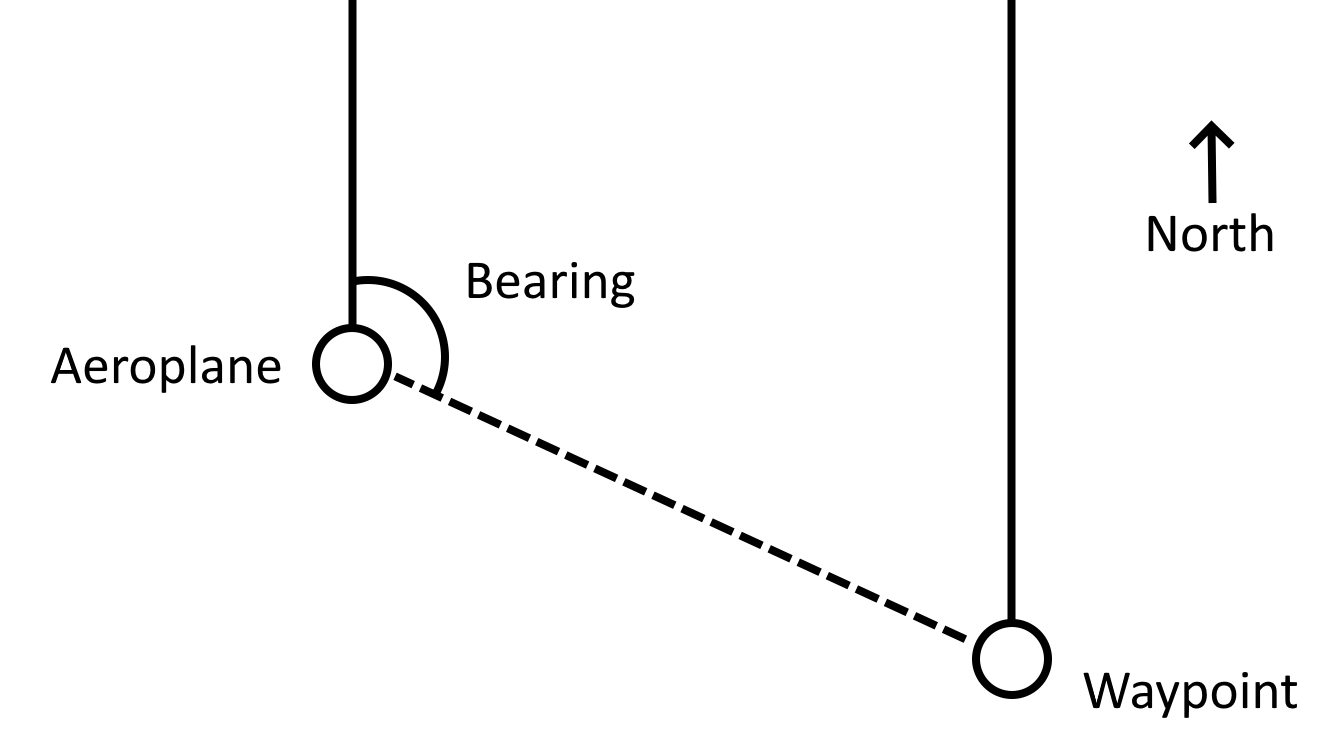
\includegraphics{diagrams/directto.png}
\caption{\label{fig:directto}Relevance of bearing in flying to a point}
\end{figure}

\begin{figure}[H]
\centering
\begin{tabular}{ |l| } 
\hline
\multicolumn{1}{ |c| }{\textbf{Direct : LateralMode}} \\
\hline
Waypoint waypoint \\
\hline
float TrackDelta() \\
override float RollCommand() \\
override LateralMode? NewMode() \\
\hline
\end{tabular}
\caption{\label{fig:directmodeclass}Direct mode class diagram}
\end{figure}

\paragraph{Testing}
All of these subsystems will have to be tested as they are developed.
The following data should be used during the iterative development:
\begin{itemize}
    \item The altitude change modes should be tested by giving instructions with varying differences in height from the aeroplane's current height, for example giving an instruction to climb to the altitude the aeroplane is already at or close to, or very far from, to ensure it acts correctly.
    \item The glideslope simulation should be tested with a variety of different glideslope angles, from 3 to 5 degrees, to confirm it can handle all of them.
    The aeroplane should be flown towards it at different airspeeds within a realistic range such as between 180 and 200 knots.
    \item The heading select mode should be tested by giving a range of different headings and confirming it always turns in the quickest direction when told to.
    Behaviour should also always be consistent when for example giving an instruction to fly a heading the aeroplane is already on or close to.
    \item To test the localizer, the aeroplane should be flown towards it at different plausible angles and airspeeds to confirm it behaves realistically when having to make a sharper turn.
    \item To test the direct to waypoint functionality, the aeroplane should be instructed to fly to waypoints that are in a variety of different positions relative to it and its direction of travel.
    This would confirm that it is capable of for example making a 180-degree turn to fly towards a waypoint which is behind it.
\end{itemize}


\subsection{Interface}
Because it is effective in ATC-Sim (section \ref{atc-sim}), the simulator will have two main screens: a main menu where the user can select which airport they want to control at, and a separate gameplay screen they will be taken to where that will take place.
Each will be a separate 'scene' in Godot, which can be created independently.

\subsubsection{Main menu}
\begin{figure}[H]
\centering
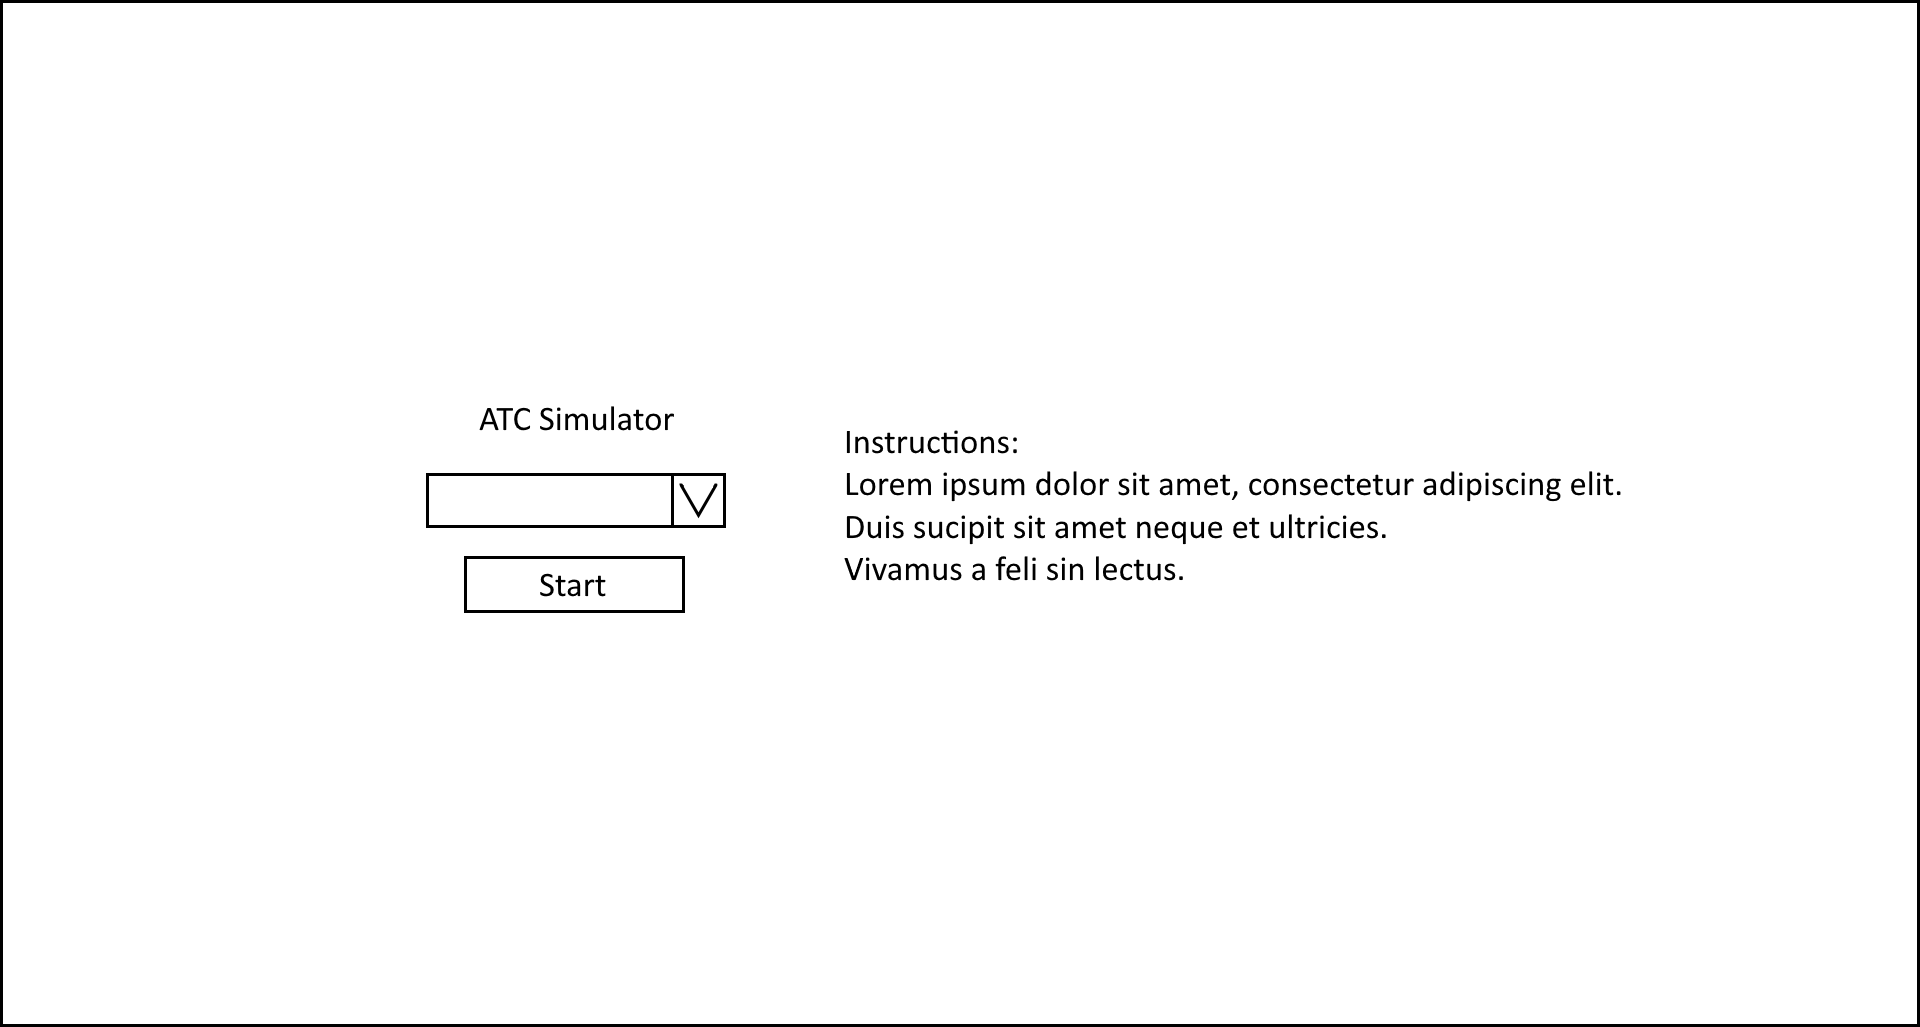
\includegraphics[width=\textwidth]{diagrams/mainmenu.png}
\caption{\label{fig:main_menu_design}Main menu screen design}
\end{figure}

Figure \ref{fig:main_menu_design} shows an approximate and simple design for a main menu.
A dropdown menu will be present which will be populated with the airport options available stored on the computer, with one of them selected by default.
A button directly below it will initiate the gameplay.
This should be fairly intuitive and usable.
Some text can be shown to give some help with how to use the simulation.

\subsubsection{Aeroplanes}
The interface for the aeroplanes comprises both displaying the necessary information about them, and being able to give instructions to them.
As described in section \ref{existingsolutions}, there are various approaches to giving instructions to the aeroplanes.
One is to use text input.
The problem with this is that, especially for users who are slow at typing, it may be slow to use; also the user could make a typo which would require them to type the instruction out again.
Another approach is to use mouse movements.
This would be faster and more intuitive to use but would compromise on realism and might not enable me to offer the complex set of instructions necessary.
Therefore to strike the best balance between usability and realism, I will use a system in which the user enters values into input boxes on a tag next to the aeroplane.
The tag will serve the dual purpose of displaying information and allowing the user to give instructions.

Figure \ref{fig:aeroplane_design} shows the four main features of the aeroplane interface.
\begin{itemize}
    \item The blip: a dot or other symbol showing the last known position of the aeroplane, which the other features are centred around.
    \item The leader line: a line pointing in the last known direction of travel.
    \item History dots: a series of dots or other symbols showing the previously received positions of the aeroplane, illustrating its motion.
    \item The tag: a box which can be dragged around relative to the blip showing information about the aeroplane; it will also be used to give instructions to the aeroplane.
\end{itemize}

The input boxes on the tag will check if the user's input is an integer, within a reasonable range, before sending the appropriate instruction event to the aeroplane simulation.
When e.g. an altitude is assigned with the input box, the value inputted will remain there so that the user can see what altitude they assigned.
If the user's input is invalid, or they click away from the field before sending the instruction by pressing enter, it will revert the contents of the input box to before the user started editing it.

\begin{figure}[H]
\centering
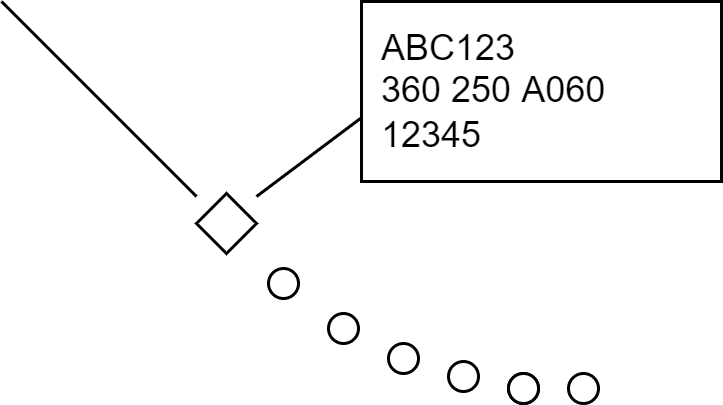
\includegraphics[width=0.5\textwidth]{diagrams/aeroplane_design.png}
\caption{\label{fig:aeroplane_design}Design of the aeroplane display}
\end{figure}

The position of the aeroplane display on the screen will be separated from the physical position of the aeroplane in the simulation, and calculated by multiplying that position by the scale factor.
This also enables the functionality of the position of the aircraft only updating every 4 seconds while the actual position is still constantly changing, by keeping a copy of the last updated position in an attribute displayPositionNm (figure \ref{fig:aeroplanedisplayclass}).

\begin{figure}[H]
\centering
\begin{tabular}{ |l| } 
\hline
\multicolumn{1}{ |c| }{\textbf{AeroplaneDisplay}} \\
\hline
Aeroplane aeroplane \\
Vector2 displayPositionNm \\
\hline
\end{tabular}
\caption{\label{fig:aeroplanedisplayclass}Aeroplane display class diagram}
\end{figure}

\paragraph{Usability}
\begin{itemize}
    \item Tooltips on each input field or text label on the aeroplane tag will be shown so that the user can easily see what they show or what their purpose is.
    \item Any inputs to the input boxes should be expected to be in units familiar to the user, for example the altitude field will accept a number in hundreds of feet.
    \item To make the aeroplane tag more usable, the user should be able to use the tab key to cycle through the available input boxes.
    This means they have to move between using the keyboard and the mouse less, saving time when making instructions.
\end{itemize}

\paragraph{Testing}
During development, the input validation should be tested with a variety of different normal, boundary, and error values.
For example 0, 360, 180, 361, "aaa", could be entered into the heading field.
After development, the time it takes to make an instruction should be measured to see if the success criteria have been achieved.

\subsection{Traffic simulation}
The traffic simulation system will run in a loop, incrementing a timer each iteration by how much time has passed since the previous iteration.
It will then check if that time has exceeded the configured time interval for an arrival aeroplane appearing, and reset the timer before doing that if so.
A list of entry points defined by a waypoint and an altitude will be configured for each airport at which the system will add an aeroplane.
All added aeroplanes 

The same system will be used to add departing aeroplanes, which will be added from a runway selected by the user.
Departing aeroplanes will be randomly assigned one of certain exit waypoints which the user will have to guide them to, similarly to a successful feature of ATC-Sim (section \ref{atc-sim}) which creates interesting scenarios.

\subsection{Terrain drawing}
When the user first starts the simulation at an airport, the system will loop through the coastline data associated with the airport (stored in GeoJSON format\footnote{\url{https://en.wikipedia.org/wiki/GeoJSON}}, consisting of LineStrings) calculating the relative position in nautical miles of the coordinates from the reference point, storing them in a list.
This can be done once at the start to save performance because it only has to be calculated once.
Then to draw the lines on the screen this list will be iterated through, and the values will be multiplied by the scale.
When the scale changes, they must then be re-drawn from this list.

\paragraph{Testing}
During development, data for a small geographical area should be inputted to more easily see problems, and larger areas to validate it functions properly.


\subsection{Waypoints}
\begin{figure}[H]
\centering
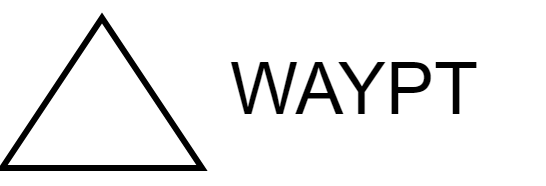
\includegraphics{diagrams/waypointdesign.png}
\caption{\label{fig:waypointdesign}Waypoint design}
\end{figure}

Waypoints should appear on the screen as in the diagram, with a symbol depending on their type and text with their name next to them.
Data about their position, type, and name will need to be stored.
When the user first starts the simulation at a particular airport, the system will loop through all the stored waypoints for that airport and add them to a list that can be accessed by the aeroplanes to implement their direct to waypoint navigation functionality.
Each waypoint will individually adjust their position when the scale changes to keep themselves in an accurate position on the screen, improving greatly on their implementation in ATC-Sim (section \ref{atc-sim}).

\paragraph{Testing}
This system should be tested during development with a smaller, example set of waypoints of different types, so their positions relative to each other can be confirmed.
A larger set can then be used to test performance.

\subsection{Extended centrelines}
The extended centrelines must be re-drawn every time the scale changes.
The main line can be drawn between a point at the threshold of the runway that the \acrshort{ils} approach is for, and a point in the direction of the heading of the runway from that point.
The length of this line will be calculated by multiplying the number of distance markers to be shown by the distance between them, to ensure that the line doesn't extend beyond or fall before any markers.
The distance markers will be shown by starting with a point at an interval along the main line, and drawing a perpendicular line.

\paragraph{Testing}
The input to this system is a list of \acrshort{ils} approaches, so this will be used to test it.
It can then be checked that they appear in the correct position and direction.

\clearpage
\section{Development}
I have chosen to use the Godot game engine\footnote{\url{https://godotengine.org/}} to build my simulator.
It works using a system of nodes, which I can use to hold each module of my solution.


\subsection{Data}
Many problems of the solution shown require data to be stored.
This includes waypoints, geography, airports, and more.
The Godot game engine provides a feature called \textit{resources}, which are data containers that allow you to define the names and data types of fields that the resource should store; then the engine manages writing this to the disk in an appropriate place in text.

To configure the simulator for controlling at a particular airport, I created a 'Radar Config' object, as a Godot resource.
When a user selects an airport to control at, they will be selecting a radar config.
This current radar config will be stored in a singleton class accessible by all elements of the solution.
\lstset{style=csharp}
\begin{lstlisting}[caption=RadarConfig resource]
using Godot;
using System;

public partial class RadarConfig : Resource
{
    public enum Display {Width, Height}
    [Export] public RadarStyle Style;
    [Export] public int WidthNm = 60;
    [Export] public int HeightNm = 60;
    [Export] public Display FixedBy;
    [Export] public Vector2 LatLon;
}
\end{lstlisting}

\subsection{Representing space}
As described in the design section, positions will be expressed in distances in nautical miles from a reference latitude and longitude.
The lateral and vertical distances can be calculated by using an imaginary point with the latitude of the reference point and the longitude of the point.
Because the distance will always be positive, the \gls{quadrant} the point lies in relative to the reference point must be determined and the sign flipped accordingly.
In a script called Geo, I created this function to do this, where Listing \ref{lst:getdistancenm} is the implementation of GetDistanceNm:
\lstset{style=csharp}
\begin{lstlisting}[caption=Calculating the position of a point relative to another]
public static Vector2 RelativePositionNm(Vector2 position, Vector2 relativeTo)
{
    // Get the position in nautical miles of a point relative to another

    float horizontalComponent = GetDistanceNm(relativeTo.X, relativeTo.Y, relativeTo.X, position.Y);
    // Make sign negative if longitude is less than the relative to point
    horizontalComponent = position.Y < relativeTo.Y ? -horizontalComponent : horizontalComponent;

    float verticalComponent = GetDistanceNm(relativeTo.X, position.Y, position.X, position.Y);
    // Make sign negative if latitude is less than the relative to point
    verticalComponent = position.X < relativeTo.X ? -verticalComponent : verticalComponent;

    return new Vector2(horizontalComponent, verticalComponent);
}
\end{lstlisting}
\lstset{style=csharp}
\begin{lstlisting}[label={lst:getdistancenm},caption=Function to calculate great-circle distance using the spherical law of cosines]
// Average radius of the Earth in nautical miles
private const float EarthRadiusNm = 3438.175f;

public static float GetDistanceNm(float latitude, float longitude, float otherLatitude, float otherLongitude)
{
    // Get distance in nautical miles between two points

    float centralAngle = Mathf.Acos(Mathf.Sin(latitude) * Mathf.Sin(otherLatitude) + Mathf.Cos(latitude) * Mathf.Cos(otherLatitude) * Mathf.Cos(Mathf.Abs(longitude - otherLongitude)));
    return EarthRadiusNm * Mathf.DegToRad(centralAngle);
}
\end{lstlisting}

\subsubsection{Scaling}
Because the size of the game window will change based on the resolution of the user's monitor and if they resize it, the scale factor has to continually change if a fixed real-world distance is to be displayed.
It may also be useful to be able to fix the distance by either height or width.
I created this function to do so, on a singleton class called Session that can be accessed by all other elements of the solution:
\lstset{style=csharp}
\begin{lstlisting}[label={lst:scalecalc},caption=Function to calculate the scale]
public static float Scale(Rect2 viewportRect)
{
    return RadarConfig.FixedBy switch
    {
        RadarConfig.Display.Width => viewportRect.Size.x / RadarConfig.WidthNm,
        RadarConfig.Display.Height => viewportRect.Size.y / RadarConfig.HeightNm,
        _ => throw new NotImplementedException()
    };
}
\end{lstlisting}
The position in nautical miles can then be multiplied by this value to get the position in pixels.
Here I also make the longitude or vertical component negative because in Godot, increasing values on the y-axis go down the screen.
\begin{lstlisting}[caption=Function to scale a position in nautical miles to the screen]
public static Vector2 ScaledPosition(Vector2 position, Rect2 viewportRect)
{
    return new Vector2(position.x, -position.y) * Scale(viewportRect);
}
\end{lstlisting}

\subsubsection{Pan and zoom}
To implement panning, I added a script to the virtual camera in the scene.
\lstset{style=csharp}
\begin{lstlisting}[caption=Camera panning script]
public partial class CameraPanning : Camera2D
{
    private Vector2 _initialCameraPosition;
    private Vector2 _initialMousePosition;

    public override void _Process(double delta)
    {
        if (Input.IsActionJustPressed("Reset Camera"))
        {
            Position = Vector2.Zero;
            _initialCameraPosition = Vector2.Zero;
            _initialMousePosition = GetViewport().GetMousePosition();
        }

        // Set reference points for movement
        if (Input.IsActionJustPressed("Pan Camera"))
        {
            _initialMousePosition = GetViewport().GetMousePosition();
            _initialCameraPosition = Position;
        }

        // Move the camera in the opposite direction to mouse movement, from the reference point
        if (Input.IsActionPressed("Pan Camera"))
        {
            Vector2 mouseDelta = GetViewport().GetMousePosition() - _initialMousePosition;
            Vector2 inverse = new Vector2(-mouseDelta.x, -mouseDelta.y);
            Position = _initialCameraPosition + inverse;
        }
    }
}
\end{lstlisting}
To implement zooming, I initially added the input handling to the singleton class accessible by all elements of the solution (Listing \ref{lst:zoominginput}) and modified the scale calculation function (first shown in Listing \ref{lst:scalecalc}) to include the zoom value (Listing \ref{lst:zoomscalecalc}).
I later moved the input handling to the script on the camera (which I renamed to CameraPanAndZoom) to keep the two related features in the same place.
\lstset{style=csharp}
\begin{lstlisting}[label={lst:zoominginput},caption=Camera zooming]
public override void _Input(InputEvent inputEvent)
{
    if (inputEvent.IsActionPressed("Zoom In"))
    {
        _zoom *= (1f + ZoomSpeed);
    }
    else if (inputEvent.IsActionPressed("Zoom Out"))
    {
        _zoom *= (1f - ZoomSpeed);
    }
    else if (inputEvent.IsActionPressed("Reset Camera"))
    {
        _zoom = 1f;
    }
    _zoom = Mathf.Clamp(_zoom, 0.1f, 10f);
}
\end{lstlisting}
\lstset{style=csharp}
\begin{lstlisting}[label={lst:zoomscalecalc},caption=Scale calculation with zoom]
return RadarConfig.FixedBy switch
{
    RadarConfig.DisplayFixedBy.Width => (viewportRect.Size.x / RadarConfig.WidthNm) * _zoom,
    RadarConfig.DisplayFixedBy.Height => (viewportRect.Size.y / RadarConfig.HeightNm) * _zoom,
    RadarConfig.DisplayFixedBy.Compromise => (viewportRect.Size.x / RadarConfig.WidthNm + viewportRect.Size.y / RadarConfig.HeightNm) / 2 * _zoom,
    _ => throw new NotImplementedException()
};
\end{lstlisting}
Upon testing, I found that when zooming in and out the camera appeared to move laterally: it did not zoom in towards the centre of the screen.
To fix this I realized I had to scale up or down the position of the camera as the user zoomed in or out.
\lstset{style=csharp}
\begin{lstlisting}[caption=Modified zoom function to scale position]
public override void _Input(InputEvent inputEvent)
{
    if (inputEvent.IsActionPressed("Zoom In"))
    {
        Simulator.Zoom *= (1f + Simulator.ZoomSpeed);
        Position *= (1f + Simulator.ZoomSpeed);
        SetReference();
    }
    else if (inputEvent.IsActionPressed("Zoom Out"))
    {
        Simulator.Zoom *= (1f - Simulator.ZoomSpeed);
        Position *= (1f - Simulator.ZoomSpeed);
        SetReference();
    }
    else if (inputEvent.IsActionPressed("Reset Camera"))
    {
        Simulator.Zoom = 1f;
    }
}
\end{lstlisting}
I also discovered that as I zoomed in the speed of the zooming increased, and as I zoomed out it decreased.
To fix this and meet the success criteria, I changed how the zoom is calculated, simultaneously making it be in fixed steps so that when getting to the minimum or maximum values, no inconsistency is caused by rounding.
\lstset{style=csharp}
\begin{lstlisting}[caption=Zooming in increments]
public override void _Input(InputEvent @inputEvent)
{
    if (@inputEvent.IsActionPressed("Zoom In"))
    {
        if (Simulator.Zoom < MaxZoom)
        {
            Simulator.Zoom++;
            // Move the camera to compensate for stretching of distances
            Position *= 1f + Simulator.ZoomSpeed;
            SetReference();
        }
    }
    else if (@inputEvent.IsActionPressed("Zoom Out"))
    {
        if (Simulator.Zoom > MinZoom)
        {
            Simulator.Zoom--;
            // Move the camera to compensate for stretching of distances
            Position /= 1f + Simulator.ZoomSpeed;
            SetReference();
        }
    }
    else if (@inputEvent.IsActionPressed("Reset Camera"))
    {
        Simulator.Zoom = 0;
    }
}
\end{lstlisting}
\lstset{style=csharp}
\begin{lstlisting}[caption=New calculation of zoom value in scale function]
// Calculate zoom value from increment
float zoomValue = Mathf.Pow(1 + ZoomSpeed, Zoom);
return RadarConfig.FixedBy switch
{
    RadarConfig.DisplayFixedBy.Width => (viewportRect.Size.X / RadarConfig.WidthNm) * zoomValue,
    RadarConfig.DisplayFixedBy.Height => (viewportRect.Size.Y / RadarConfig.HeightNm) * zoomValue,
    RadarConfig.DisplayFixedBy.Compromise => (viewportRect.Size.X / RadarConfig.WidthNm + viewportRect.Size.Y / RadarConfig.HeightNm) / 2 * zoomValue,
    _ => throw new NotImplementedException()
};
\end{lstlisting}
Testing the feature again after making these changes revealed the problems had been resolved.

\subsection{Terrain drawing}
To implement this feature, I added a 2D node in the gameplay scene in Godot and added the script below.
OnScaleChanged is called every time the scale changes, which necessitates re-drawing.
\lstset{style=csharp}
\begin{lstlisting}[caption=Geography drawing script]
public partial class DrawGeography : Node2D
{
	private readonly List<List<Vector2>> _polyLines = new();

	public override void _Ready()
	{
		// Read GeoJSON polylines
		var polyLines = Json.ParseString(Simulator.RadarConfig.GeoLines.data).AsGodotArray();
		foreach (var polyLine in polyLines)
		{
			// Get the relative position of each point in the polyline
			List<Vector2> points = new();
			foreach (float[] point in polyLine.AsGodotArray())
			{
				Vector2 PointNm = Geo.RelativePositionNm(new Vector2(point[1], point[0]), Simulator.RadarConfig.LatLon);
				points.Add(PointNm);
			}
			_polyLines.Add(points);
		}
	}

	public override void _Draw()
	{
		GD.Print("Drawing terrain");
		foreach(List<Vector2> polyLine in _polyLines)
		{
			// Scale the points in the line
			Vector2[] scaledPolyline = polyLine.Select(PointNm => Simulator.ScaledPosition(PointNm, GetViewportRect())).ToArray();
			DrawPolyline(scaledPolyline, Simulator.RadarConfig.Style.CoastlineColour);
		}
	}

	public void OnScaleChanged()
	{
		QueueRedraw();
	}
}
\end{lstlisting}
Upon testing this, I noticed that beyond a certain distance the terrain started to show up incorrectly, seeming to begin to be mirrored laterally.
I could not find anything wrong with the terrain drawing code itself, rather it turned out that the problem was with the distance calculation (which had previously appeared to work perfectly with the other elements of the solution): the latitudes and longitudes had to be converted from degrees to radians.
I therefore modified this function as below.
\lstset{style=csharp}
\begin{lstlisting}[caption=Modified distance function]
public static float GetDistanceNm(float latitude, float longitude, float otherLatitude, float otherLongitude)
{
    // Convert to radians
    float lat = Mathf.DegToRad(latitude);
    float lon = Mathf.DegToRad(longitude);
    float otherLat = Mathf.DegToRad(otherLatitude);
    float otherLon = Mathf.DegToRad(otherLongitude);
    
    float centralAngle = Mathf.Acos(Mathf.Sin(latitude) * Mathf.Sin(otherLatitude) + Mathf.Cos(latitude) * Mathf.Cos(otherLatitude) * Mathf.Cos(Mathf.Abs(longitude - otherLongitude)));
    return EarthRadiusNm * Mathf.DegToRad(centralAngle);
}
\end{lstlisting}
Upon further testing, this appeared to resolve the problem.
However, when testing with a different set of coastline data from another part of the world, a bizarre problem appeared: it looked like the points of the lines drawn were rounded onto a grid.
I could not determine exactly why this was, but using a different formula for the distance calculation resolved this.
\lstset{style=csharp}
\begin{lstlisting}[caption=Final distance function with the Haversine formula]
public static float GetDistanceNm(float latitude, float longitude, float otherLatitude, float otherLongitude)
{
    // Convert to radians
    float lat = Mathf.DegToRad(latitude);
    float lon = Mathf.DegToRad(longitude);
    float otherLat = Mathf.DegToRad(otherLatitude);
    float otherLon = Mathf.DegToRad(otherLongitude);
    // Use the haversine formula
    float haversineTheta = Haversine(otherLat - lat) + Mathf.Cos(lat) * Mathf.Cos(otherLat) * Haversine(otherLon - lon);
    return EarthRadiusNm * Archaversine(haversineTheta);
}
\end{lstlisting}

\subsection{Waypoints}
To implement this feature I first created a Godot resource to store the information about waypoints.
\lstset{style=csharp}
\begin{lstlisting}[caption=Waypoint data resource]
public partial class WaypointData : Resource
{
    public enum Type {RNAV, VORDME, VOR, NDB}
    [Export] public Type Basis;
    [Export] public Vector2 LatLon;
}
\end{lstlisting}
I then created a waypoint scene with a 2D sprite root node and a label node attached.
\begin{figure}[H]
\centering
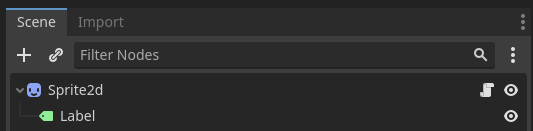
\includegraphics[width=0.7\textwidth]{screenshots/wptree.png}
\caption{\label{fig:wpscenetree}Waypoint scene tree}
\end{figure}
I attached the below script to the root node of the waypoint scene.
\lstset{style=csharp}
\begin{lstlisting}[caption=Waypoint script]
public partial class Waypoint : Sprite2D
{
    public WaypointData WaypointData;
    public Vector2 PositionNm;

    public override void _Ready()
    {
        // Set icon coressponding to waypoint type
        Texture = WaypointData.Basis switch
        {
            WaypointData.Type.RNAV => Simulator.RadarConfig.Style.RNAVTexture,
            WaypointData.Type.VOR => Simulator.RadarConfig.Style.VORTexture,
            WaypointData.Type.VORDME => Simulator.RadarConfig.Style.VORDMETexture,
            WaypointData.Type.NDB => Simulator.RadarConfig.Style.NDBTexture,
            _ => throw new NotImplementedException()
        };

        // Set name
        GetChild<Label>(0).Text = WaypointData.ResourceName;

        // Calculate position relative to screen centre
        PositionNm = Geo.RelativePositionNm(WaypointData.LatLon, Simulator.RadarConfig.LatLon);
    }

    public override void _Draw()
    {
        Position = Simulator.ScaledPosition(PositionNm, GetViewportRect());
    }

    public void OnScaleChanged()
    {
        QueueRedraw();
    }
}
\end{lstlisting}
I then created an empty node in the gameplay scene with the script below attached, to serve the purpose of adding all the waypoints from the configuration, instantiating the waypoint scene for each and adding them as children (see Figure \ref{fig:wpscenetree2}).
\lstset{style=csharp}
\begin{lstlisting}[caption=Waypoints management script]
public partial class Waypoints : Node
{
    [Export] public Resource WaypointScene;

    public override void _Ready()
    {
        PackedScene waypointScene = GD.Load<PackedScene>(WaypointScene.ResourcePath);
        Simulator.Waypoints.Clear();
        // Add all the waypoints for the radar config to the scene
        foreach (WaypointData waypointData in Simulator.RadarConfig.Waypoints)
        {
            Node node = waypointScene.Instantiate();
            Waypoint waypoint = (Waypoint)node;
            waypoint.WaypointData = waypointData;
            node.Name = waypointData.ResourceName;
            AddChild(node);
            // Register waypoint
            Simulator.Waypoints.Add(waypointData.ResourceName, waypoint);
        }
    }
}
\end{lstlisting}
\begin{figure}[H]
\centering
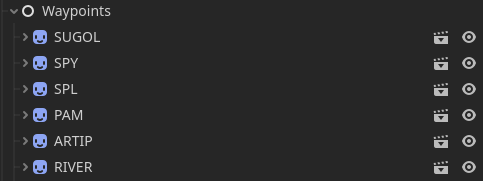
\includegraphics[width=0.7\textwidth]{screenshots/wptree2.png}
\caption{\label{fig:wpscenetree2}Waypoints scene tree in the gameplay scene}
\end{figure}
To test this I compared the result with maps of the waypoints and they all appeared in the correct places, and stayed in the correct places when zooming in and out.

\subsection{Simulated aeroplanes}
Godot has a feature called scenes which allows a tree of nodes to be stored which can be instantiated later.
Each node can have a script attached to it.
In my solution, each aeroplane will be an instance of an aeroplane scene with the primary script controlling it being on the root node.

\subsubsection{Physics simulation}\label{physicssimulation}
Listing \ref{lst:aeroplanescript} shows the main script I created to run on the root node of the aeroplane scene.
It shows the attributes and the validation on the heading.
Scripts on Godot nodes inherit from a parent Node class, and can then override built-in methods such as PhysicsProcess which is called every physics step.
This is part of the 'game loop'.
\lstset{style=csharp}
\begin{lstlisting}[label={lst:aeroplanescript}, caption=The aeroplane script]
public partial class Aeroplane : Node
{
    public const int SecondsInAnHour = 3600;

    [Export] public float Altitude;
    [Export] public float TrueAirspeed;
    private float _heading;
    [Export] public float TrueHeading
    {
        get => _heading;
        set => _heading = Mathf.Wrap(value, 0, 360);
    }

    [Export] public Vector2 PositionNm;
    [Export] public Vector2 Velocity;

    public override void _PhysicsProcess(double delta)
    {
        Vector2 airVector = HeadingToVector(TrueHeading) * TrueAirspeed;
        Vector2 windVector = HeadingToVector(Session.WindDirection) * Session.WindSpeed;
        // Add vectors and convert from nautical miles/hour to /second
        // then multiply by elapsed number of seconds this iteration
        Velocity = (airVector + windVector) / SecondsInAnHour * (float)delta;
        PositionNm += Velocity;
    }
}
\end{lstlisting}

To convert a \gls{heading} to a \gls{directionvector} it is necessary to determine which \gls{quadrant} the \gls{heading} lies in.
The angle the \gls{heading} makes with the $y$ axis can then be calculated.
Then the sine rule can be used to calculate the positive $x$ and $y$ components of a \gls{unitvector} with that angle.
Knowing which \gls{quadrant} the \gls{heading} lies in, the sign of the components can be changed appropriately by multiplying each by $1$ or $-1$.
\lstset{style=csharp}
\begin{lstlisting}[caption=Converting a heading to a vector]
private Vector2 HeadingToVector(float heading)
{
  Vector2 quadrant = new Vector2(1, 1);
  float theta = heading;
  if (heading > 270)
  {
    theta = 360 - heading;
    quadrant = new Vector2(-1, 1);
  }
  else if (heading > 180)
  {
    theta = heading - 180;
    quadrant = new Vector2(-1, -1);
  }
  else if (heading > 90)
  {
    theta = 180 - heading;
    quadrant = new Vector2(1, -1);
  }
  return new Vector2(Mathf.Sin(Mathf.DegToRad(theta)), Mathf.Sin(Mathf.DegToRad(90 - theta))) * quadrant;
}
\end{lstlisting}
To test the physics simulation and its wind drift simulation, I needed to be able to see a clear indication of the aeroplane's movement, so I chose to add the leader line at this point (development of this is described in section \ref{leaderline}).

\paragraph{Testing}
Without a system for controlling the addition of more aeroplanes I initially just used one instance of the aeroplane class which I could easily control.
To enable the testing of the physics simulation without an implemented system for instructions or getting live weather information, I created a temporary menu interface with three sliders: one for wind speed, wind direction, and aeroplane heading, shown in Figure \ref{fig:winddebug}.
\begin{figure}[H]
\centering
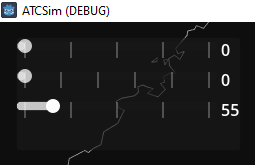
\includegraphics{screenshots/winddebug.png}
\caption{\label{fig:winddebug}Wind and heading debug menu}
\end{figure}
Using this tool, I set different parameters as defined in the design section and observed that the leader line indicated an accurate looking affect on the direction of travel.

\subsubsection{Navigation simulation}
To begin implementing this feature, I created a Guidance script in the same folder as the Aeroplane script.
I first implemented the lateral guidance modes, adding the below base classes and a variable on the Aeroplane class with the type LateralMode as per the design.
\lstset{style=csharp}
\begin{lstlisting}[caption=Guidance base classes]
public class Mode
{
    protected Aeroplane _aeroplane;
}

public class LateralMode : Mode
{
    public virtual float RollCommand()
    {
        return 0f;
    }
}
\end{lstlisting}
Because it is not possible to easily test the guidance features without being able to give the instructions they correspond to, I developed the interfaces for each first (section \ref{thetag}).

\paragraph{Heading select}
At the same time as adding the heading field to the tag, I added a receiver function for the instructions on the Aeroplane class.
\lstset{style=csharp}
\begin{lstlisting}[caption=Heading instruction receiver function]
private void OnHeadingInstruction(float heading, int turnDirection)
{
    _lateralGuidanceMode = new Guidance.HeadingSelect(this, heading, (Guidance.TurnDirection)turnDirection);
}
\end{lstlisting}
I chose to implement the heading select mode first because it is one of the most fundamental.
The listing below shows my implementation of the heading select mode design.
\lstset{style=csharp}
\begin{lstlisting}[caption=Heading select guidance mode and turn direction enum]
public enum TurnDirection
{
    Left,
    Right,
    Quickest
}

public class HeadingSelect : LateralMode
{
    private float _selectedHeading;
    private TurnDirection _turnDirection;

    private float HeadingDelta(TurnDirection direction)
    {
        // Find the angle in degrees between the aircraft's current heading and the selected heading, assuming a turn in a given direction.
        float headingDelta = direction == TurnDirection.Left ? _aeroplane.TrueHeading - _selectedHeading : _selectedHeading - _aeroplane.TrueHeading;
        if (headingDelta < 0)
        {
            headingDelta += 360;
        }
        return headingDelta;
    }

    public override float RollCommand()
    {
        // If the difference between the current and selected heading is greater than that needed to roll out,
        if (HeadingDelta(_turnDirection) > (_aeroplane.Roll / Aeroplane.RollRate) * _aeroplane.Roll + 0.01f)
        {
            // Command a standard rate turn in the appropriate direction
            return _turnDirection == TurnDirection.Right ? Aeroplane.StandardRateTurn : -Aeroplane.StandardRateTurn;
        }
        else
        {
            return 0f;
        }
    }

    public HeadingSelect(Aeroplane aeroplane, float heading, TurnDirection turnDirection)
    {
        _aeroplane = aeroplane;
        _selectedHeading = heading;
        if (turnDirection == TurnDirection.Quickest)
        {
            // Find which direction it would be quicker to turn in to reach the selected heading
            _turnDirection = HeadingDelta(TurnDirection.Left) < HeadingDelta(TurnDirection.Right) ? TurnDirection.Left : TurnDirection.Right;
        }
        else
        {
            _turnDirection = turnDirection;
        }
    }
}
\end{lstlisting}

\paragraph{Localizer}
To implement this feature I started by creating a prototype in Julia, that allowed me to quickly adjust the PID controller parameters and see a plot of the result.
\lstset{style=csharp, language=Julia}
\begin{lstlisting}[label={lst:pidlocsim}, caption=PID Localizer Simulation test script]
roll_rate = 0.5
seconds_in_an_hour = 3600
localiser_heading = 90

aircraft = Aircraft(180, 130, 0, Point(-1, 0.3))
controller = PIDController(15.5, 0, 200, 0, 0)

for i in 0:(2 * 60 / delta)
    deviation = deviation_feet(aircraft)
    command = iterate(controller, delta, 0, deviation)
    if abs(deviation) < 0.25
        aircraft.roll = move_towards(aircraft.roll, command, roll_rate * delta)
    end
    aircraft.heading += aircraft.roll * delta;

    air_vector = heading_to_vector(aircraft.heading) * aircraft.airspeed
    wind_vector = heading_to_vector(180) * 0
    ground_vector = (air_vector + wind_vector) / seconds_in_an_hour * delta
    aircraft.position.x += ground_vector[1]
    aircraft.position.y += ground_vector[2]
end
\end{lstlisting}
Once I had confirmed this design, I created the localizer lateral guidance mode class.
To increase the flexibility of the navigation system, I at this point enabled guidance modes to be armed and activated when their Activate method returns true.
\lstset{style=csharp}
\begin{lstlisting}[caption=Approach instruction receiver on Aeroplane class]
private void OnApproachInstruction(int approach_index)
{
    Approach = Simulator.EnabledILSApproaches[approach_index];
    ArmedLateralGuidanceModes.Add(new Localiser(this));
    ArmedVerticalGuidanceModes.Add(new Glideslope(this));
    GD.Print("Cleared ", Approach.ResourceName, " approach!");
}
\end{lstlisting}
\lstset{style=csharp}
\begin{lstlisting}[caption=Localizer guidance mode class]
public class Localiser : IArmableLateralMode
{
    private readonly Aeroplane _aeroplane;
    private readonly PIDController _controller = new(15.5f, 0, 300);

    private float Deviation()
    {
        ILSApproach approach = _aeroplane.Approach;
        Vector2 locPosition = RelativePositionNm(approach.LocaliserLatLon, Simulator.RadarConfig.LatLon);
        float distance = _aeroplane.PositionNm.DistanceTo(locPosition);
        float bearing = Util.Bearing(_aeroplane.PositionNm, locPosition);
        float angularDeviation = approach.LocaliserHeading - bearing;
        float deviation = Mathf.Sin(Mathf.DegToRad(angularDeviation)) * distance;
        return deviation;
    }

    public bool Activate()
    {
        return Mathf.Abs(Deviation()) < 0.25;
    }

    public float RollCommand(float delta)
    {
        return _controller.Iterate(delta, 0, Deviation());
    }

    public Localiser(Aeroplane aeroplane) => _aeroplane = aeroplane;
}
\end{lstlisting}

\paragraph{Glideslope}
Because it would be difficult to add the debugging features necessary to the main project, I chose to create a prototype python program, shown in Listing \ref{lst:pidilssim}, that would run a simplified simulation (using the only two dimensions which are important: distance from the transmitter and height) and allow me to more quickly iterate on the glideslope vertical mode design and see the result.
I slightly changed the original design to only iterate the PID controller and start issuing commands once within a certain vertical deviation of the glideslope.

\lstset{style=csharp, language=Python}
\begin{lstlisting}[label={lst:pidilssim}, caption=PID ILS Simulation test script]
controller = PIDController(0.02, -0.0005, 0.3)
control = False

for i in range(int((6 * 60) / DELTA)):
    glideslope_height = np.absolute(distance) * NM_TO_FEET * maths.tan(maths.radians(glideslope_angle))
    glideslope_deviation = height - glideslope_height

    # Start controlling if within 250 feet of the glideslope
    control += np.absolute(glideslope_deviation) < 250

    if control:
        fpa_command = controller.iterate(DELTA, 0, glideslope_deviation)
    else:
        fpa_command = 0

    fpa = move_towards(fpa, fpa_command, PITCH_RATE * DELTA)
    height += airspeed * maths.sin(maths.radians(fpa)) * KNOTS_TO_FPS * DELTA

    # Update position
    distance += airspeed * maths.cos(np.absolute(maths.radians(fpa))) / SECONDS_IN_AN_HOUR * DELTA

    if height <= 30:
        break
\end{lstlisting}
I used this program to easily generate plots of the aeroplane and the glideslope's height, and the commanded flight path angle, with respect to the aeroplane's distance from the glideslope transmitter.
I tried tuning the PID controller parameters, but was never able to get it to reliably follow the glideslope, especially when testing with different glideslope angles and airspeeds.
Figure \ref{fig:pidilssim} shows the result of a test with the best result I was able to achieve with this method, the blue curve on the vertical axes shows the FPA commanded at each point; the straight blue line is the glideslope; and the orange line is the aeroplane, which is seen to over and undershoot the glideslope.

Therefore I created a new simpler design which would, based on the time necessary to pitch down to match the glideslope's angle, calculate the point at which to command pitch down in order to align with the glideslope's path.
This involved changing lines 11 to 14 of Listing \ref{lst:pidilssim} to this:
\lstset{style=csharp, language=Python}
\begin{lstlisting}[label={lst:ilssim}, caption=ILS Simulation test script]
if np.absolute(glideslope_deviation) * ( 1 / maths.tan(maths.radians(glideslope_angle))) < (0--glideslope_angle) / PITCH_RATE * airspeed * 0.845:
    fpa_command = -glideslope_angle
else:
    fpa_command = 0
\end{lstlisting}
I tested this change with the aeroplane at different airspeeds and the glideslope at many angles and it was always able to perform perfectly, like shown in Figure \ref{fig:ilssim}.

\begin{sidewaysfigure}
    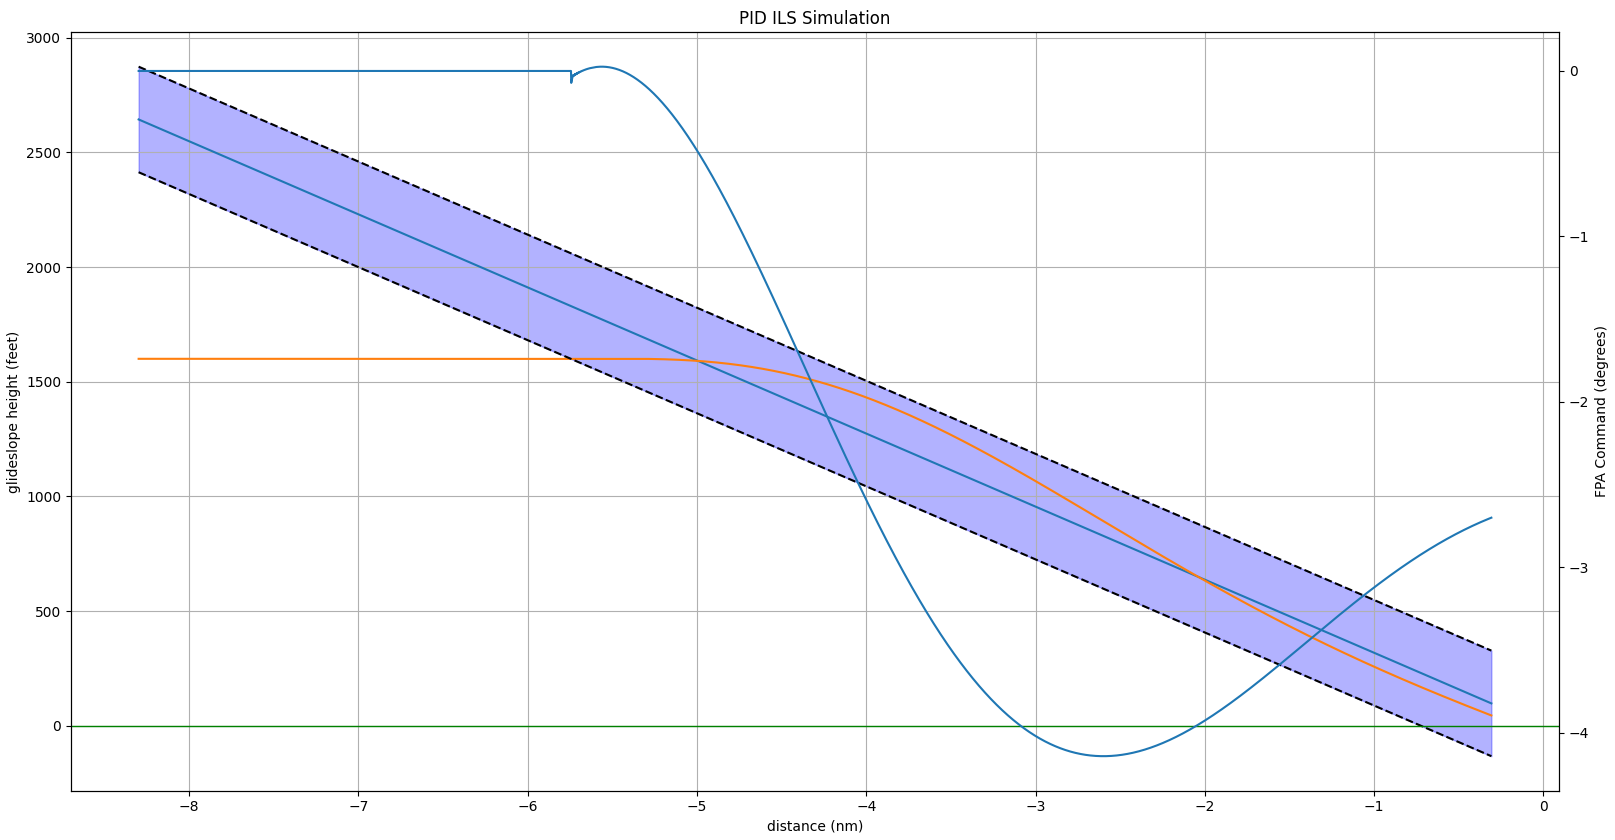
\includegraphics[width=\textwidth]{diagrams/pidilssim.png}
    \caption{\label{fig:pidilssim}PID ILS Simulation}
\end{sidewaysfigure}

\begin{sidewaysfigure}
    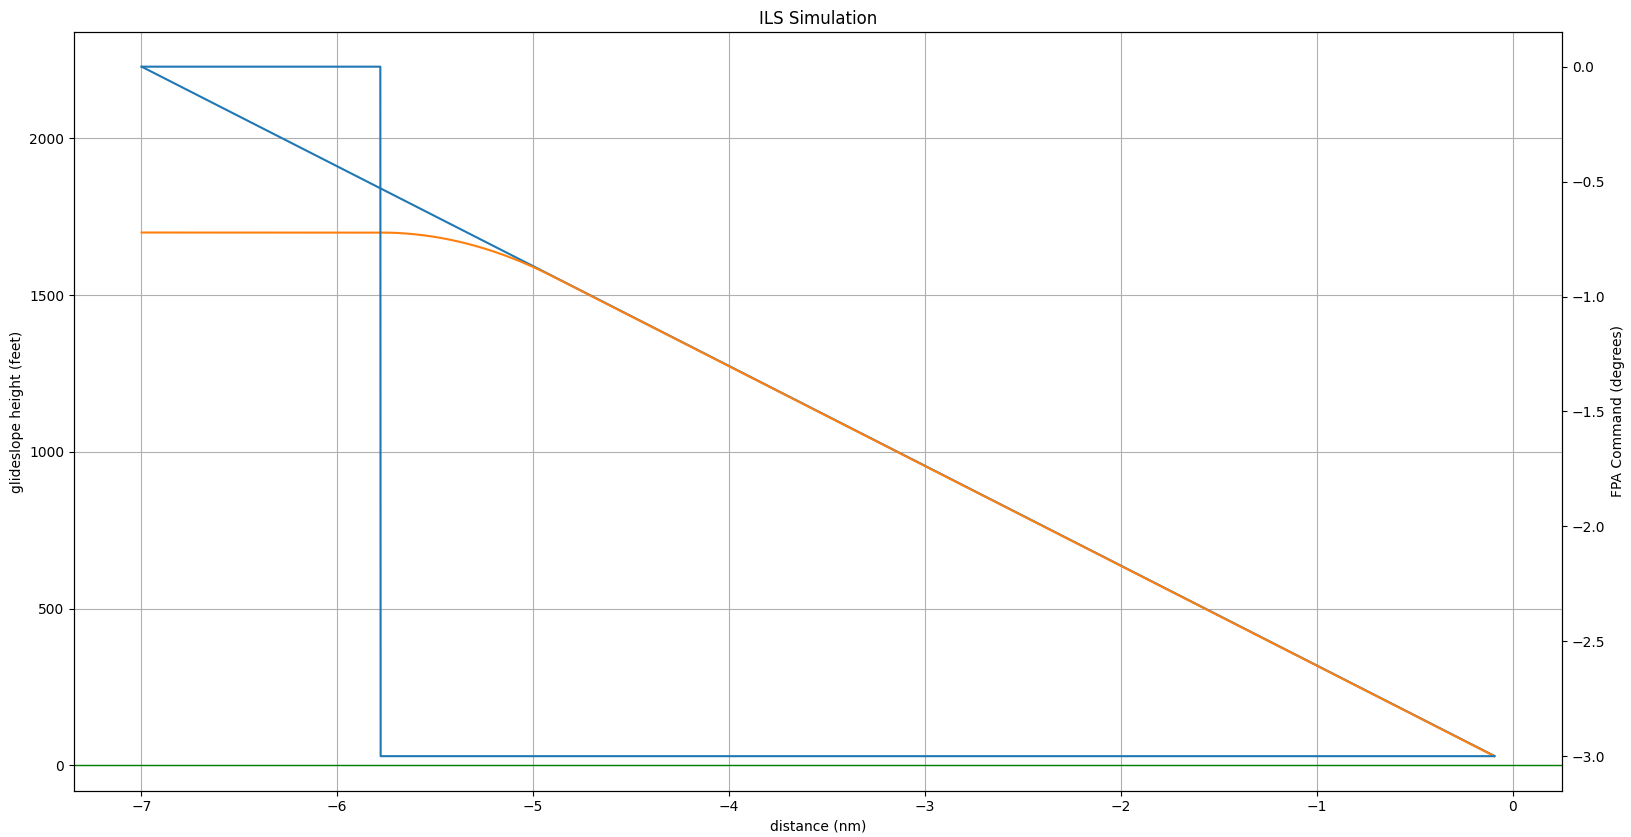
\includegraphics[width=\textwidth]{diagrams/ilssim.png}
    \caption{\label{fig:ilssim}ILS Simulation}
\end{sidewaysfigure}

\clearpage

I then created the Glideslope vertical guidance mode with this new design.
\lstset{style=csharp}
\begin{lstlisting}[caption=Glideslope vertical guidance mode]
public class Glideslope : IArmableVerticalMode
{
    private readonly Aeroplane _aeroplane;

    private float Deviation()
    {
        // Return vertical deviation from the glideslope in feet
        ILSApproach approach = _aeroplane.Approach;
        float distance = _aeroplane.PositionNm.DistanceTo(RelativePositionNm(approach.GlideslopeLatLon, Simulator.RadarConfig.LatLon));
        float glideslopeHeight = distance * Aeroplane.NauticalMilesToFeet * Mathf.Tan(Mathf.DegToRad(approach.GlideslopeAngle)) + approach.GlideslopeElevation;
        return _aeroplane.TrueAltitude - glideslopeHeight;
    }

    public bool Activate()
    {
        ILSApproach approach = _aeroplane.Approach;
        // Calculate time to pitch down
        float pitchTime = (_aeroplane.FlightPathAngle + approach.GlideslopeAngle) / Aeroplane.PitchRate * _aeroplane.TrueAirspeed * 0.845f;
        float deviation = Deviation();
        // Activate when pitching down to match the glideslope will align us with its path
        // also check that we are below the glideslope
        return Mathf.Abs(deviation) * (1 / Mathf.Tan(Mathf.DegToRad(approach.GlideslopeAngle))) < pitchTime && deviation < 0;
    }

    public float FlightPathAngleCommand()
    {
        return -_aeroplane.Approach.GlideslopeAngle;
    }

    public Glideslope(Aeroplane aeroplane) => _aeroplane = aeroplane;
}
\end{lstlisting}


\subsection{Aeroplane interface}
To implement this feature I first created a node as a child (sub) node of the root node in the Aeroplane scene in Godot (Figure \ref{fig:scenetree} shows the final state of this scene), with the script shown in Listing \ref{lst:aeroplanedisplay}.
Rather than the root node being moved, this node will move itself with the correct scaling on the screen and all subcomponents such as the blip and leader line will be child nodes of it so that they do not need to manage their own position.
This also implements the design for the actual position of the aeroplane to be separated from the display position.
DisplayUpdateTimeout is a function I configured Godot to call every 4 seconds with the DisplayUpdateTimer node.
I also call the Update function from the Ready function which Godot calls when the node first appears so that when an aeroplane is newly added to the screen, it does not wait until the first display update from the timer to move to the correct position; this was a problem I noticed when first testing it.
\begin{figure}[H]
\centering
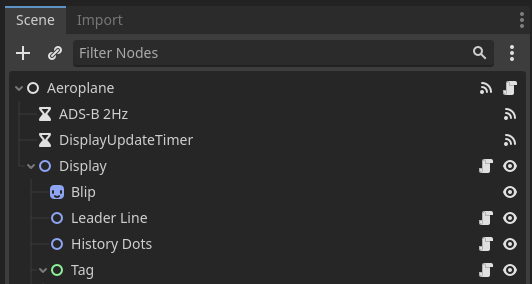
\includegraphics[width=0.7\textwidth]{screenshots/tree.png}
\caption{\label{fig:scenetree}Aeroplane scene tree}
\end{figure}
\lstset{style=csharp}
\begin{lstlisting}[label={lst:aeroplanedisplay},caption=Aeroplane display script]
public partial class AeroplaneDisplay : Node2D
{
    [Export] public Aeroplane Aeroplane;
    private Vector2 _displayPositionNm;

    private void Update()
    {
        // Sync position with aeroplane
        _displayPositionNm = Aeroplane.PositionNm;
    }

    public void DisplayUpdateTimeout()
    {
        // Update on the timeout of the display update timer
        Update();
    }

    public override void _Ready()
    {
        Update();
    }

    public override void _Process(double delta)
    {
        // Set position based on last known aeroplane position
        Position = Simulator.ScaledPosition(_displayPositionNm, GetViewportRect());
    }
}
\end{lstlisting}

\subsubsection{Leader line}\label{leaderline}
To implement this feature I created a node in the aeroplane scene as a child of the display node with the script below.
Godot calls the draw function when the texture needs to be updated.
To re-draw the line every frame so that it always shows the current heading I needed to tell Godot to execute the draw function again in an override of the Process function which is called every frame by Godot.
\lstset{style=csharp}
\begin{lstlisting}[caption=Leader line script]
public partial class LeaderLine : Node2D
{
    [Export] private Aeroplane _aeroplane;

    [Export] private Color _colour;
    [Export] private int _start = 10;
    [Export] private int _length = 40;

    private Vector2 screenVelocity;

    public override void _Draw()
    {
        // Invert the y-axis of the aeroplane's movement because the display uses an inverted y-axis
        screenVelocity = new Vector2(_aeroplane.GroundVector.X, -_aeroplane.GroundVector.Y);
        // Draw the line
        Vector2 direction = screenVelocity.Normalized();
        Vector2 start = Position + direction * _start;
        Vector2 end = start + direction * _length;
        DrawLine(start, end, _colour, -1, true);
    }

    public override void _Process(double delta)
    {
        QueueRedraw();
    }
}
\end{lstlisting}

The figure below shows this working, with the aeroplane on a heading of 55 degrees. I tested this further by changing the heading, and it rotated appropriately.
\begin{figure}[H]
\centering
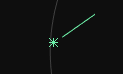
\includegraphics[]{screenshots/leaderline.png}
\caption{\label{fig:leaderline}Leader line}
\end{figure}

After I implemented the heading instruction, I wanted the leader line to only update at the same time as the position of the aeroplane, so I changed it to be linked to the same timer rather than re-drawing every frame. The figure below replaced lines 22 to 25 of the leader line script shown above.

\lstset{style=csharp}
\begin{lstlisting}[caption=Updating the leader line on a timer]
public void DisplayUpdateTimeout()
{
    QueueRedraw();
}
\end{lstlisting}

\subsubsection{The tag}\label{thetag}
In Godot, nodes are arranged to create a user interface.
The LineEdit node provides an input box and I have used it for each value on the tag.
Figure \ref{fig:tagtree} shows the final state of the scene tree of child nodes under the display node in the aeroplane scene.

In the script for each input field, the OnChanged function is called by Godot when the text is edited and OnSubmitted when the enter key is pressed.
Instructions are passed from the tag to the Aeroplane script on the root node of the scene with Godot's signals, which are essentially events which are connected between two scripts, defined using the keyword "[Signal]" in code.
I chose to use them because they are the best way of communicating between two separated modules.
I have given all input fields this code that de-focuses them when the user clicks away.
\lstset{style=csharp}
\begin{lstlisting}[caption=Input field de-focus event]
public override void _Input(InputEvent @event)
{
    // If the left mouse button is pressed outside of the field, de-focus it
    if (@event is InputEventMouseButton eventMouseButton)
        if (eventMouseButton.ButtonIndex == MouseButton.Left && eventMouseButton.Pressed == true)
            if (!GetRect().HasPoint(((InputEventMouseButton)MakeInputLocal(eventMouseButton)).Position))
                ReleaseFocus();
}
\end{lstlisting}
\begin{figure}[H]
\centering
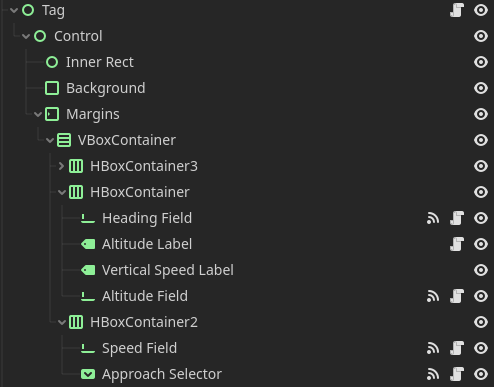
\includegraphics[width=0.7\textwidth]{screenshots/tagtree.png}
\caption{\label{fig:tagtree}Aeroplane tag scene tree}
\end{figure}


\paragraph{Heading field}
I initially implemented the heading field as below:
\lstset{style=csharp}
\begin{lstlisting}[caption=Heading field script]
public partial class HeadingField : LineEdit
{
    [Signal] public delegate void HeadingInstructionEventHandler(int heading, int turnDirection);

    public void OnChanged(string newText)
    {
        // Make all text entered uppercase
        int oldCaretColumn = CaretColumn;
        Text = newText.ToUpper();
        CaretColumn = oldCaretColumn;
    }

    public void OnSubmitted(string newText) 
    {
        // If the text entered is a valid number
        if (newText.IsValidInt())
        {
            EmitSignal(nameof(HeadingInstruction), newText.ToInt(), (int)Guidance.TurnDirection.Quickest);
            Text = newText.PadLeft(3, '0');
        }
        // If the first character is L and the rest is a valid number
        else if (newText[0] == 'L' && newText.Substring(1).IsValidInt())
        {
            EmitSignal(nameof(HeadingInstruction), newText.Substring(1).ToInt(), (int)Guidance.TurnDirection.Left);
            Text = newText.Substring(1).PadLeft(3, '0');
        }
        // If the first character is R and the rest is a valid number
        else if (newText[0] == 'R' && newText.Substring(1).IsValidInt())
        {
            EmitSignal(nameof(HeadingInstruction), newText.Substring(1).ToInt(), (int)Guidance.TurnDirection.Right);
            Text = newText.Substring(1).PadLeft(3, '0');
        }

        ReleaseFocus();
    }
}
\end{lstlisting}
I tested this with many input values as described in the design section and it worked as intended.

Then while adding the direct to waypoint navigation functionality, I added another condition to the if statement in OnSubmitted allowing the user to issue direct to instructions through the heading field by entering just its name.
At the same time I developed the feature further by making it so that the text in the input box reverts to the last valid input when entering invalid input, which I replicated across all other text input fields on the tag.
\lstset{style=csharp}
\begin{lstlisting}[caption=Heading field script]
// If the entered text is the name of a waypoint
else if (Simulator.Waypoints.ContainsKey(newText))
{
    EmitSignal(nameof(DirectInstruction), newText);
    _oldText = Text;
}
else
{
    // Cancel changes
    Text = _oldText;
}
\end{lstlisting}
\lstset{style=csharp}
\begin{lstlisting}[caption=Input field de-focus and canceling changes]
public override void _Input(InputEvent @event)
{
    // If the left mouse button is pressed outside of the field, de-focus it and cancel changes
    if (@event is InputEventMouseButton eventMouseButton)
    {
        if (eventMouseButton.ButtonIndex == MouseButton.Left && eventMouseButton.Pressed == true)
        {
            if (!GetRect().HasPoint(((InputEventMouseButton)MakeInputLocal(eventMouseButton)).Position))
            {
                ReleaseFocus();
                // Cancel changes
                Text = _oldText;
            }
        }
    }    
}
\end{lstlisting}

\paragraph{Altitude field}
Below is the implementation of the altitude field.
\lstset{style=csharp}
\begin{lstlisting}[caption=Altitude field script]
public partial class AltitudeField : LineEdit
{
    [Signal] public delegate void AltitudeInstructionEventHandler(int altitude);

    public void OnSubmitted(string newText) 
    {
        // If the text entered is a valid integer, send an instruction using that value
        if (newText.IsValidInt())
        {
            EmitSignal(nameof(AltitudeInstruction), newText.ToInt() * 100);
            Text = newText.PadLeft(3, '0');
            _oldText = Text;
        }
        else
        {
            // Cancel changes
            Text = _oldText;
        }

        ReleaseFocus();
    }
}
\end{lstlisting}

\paragraph{Speed field}
Below is the implementation of the speed field.
With this I made the addition to the design of some fields not showing unless the user hovers the mouse over the tag, because there became too many fields to show all at once.
This can be seen in the Process function.
\lstset{style=csharp}
\begin{lstlisting}[caption=Speed field script]
public partial class SpeedField : LineEdit
{
    [Signal] public delegate void SpeedInstructionEventHandler(int speed);

    [Export] private Tag _tag;
    private string _oldText = "";

    public void OnSubmitted(string newText)
    {
        // If just a number is entered e.g. 180,250
        if (newText.IsValidInt())
        {
            int speed = newText.ToInt();
            // If value is within a valid range
            if (speed > 0 && speed < 350)
            {
                EmitSignal(nameof(SpeedInstruction), speed);
                Text = newText.PadLeft(3, '0');
                _oldText = Text;
            }
        }
        else
        {
            // Cancel changes
            Text = _oldText;
        }

        ReleaseFocus();
    }

    public override void _Process(double delta)
    {
        // Hide this button if the tag isn't hovered
        if (_tag.Hovering)
        {
            Show();
        }
        else
        {
            Hide();
        }
    }
}
\end{lstlisting}

\paragraph{Approach selector}
Only during development I finalized the idea of how to fulfil the criterion of being able to give instructions to fly \acrshort{ils} approaches, and found the additional requirement of being able to cancel this instruction.
I decided to use a dropdown populated with all the enabled approaches, where selecting one from the dropdown would issue an instruction to fly that approach and selecting the first option in the dropdown which would always be text reading "Cancel" or "Unset", would cancel it.
\lstset{style=csharp}
\begin{lstlisting}[caption=Approach selector script]
public partial class ApproachSelector : OptionButton
{
    [Signal] public delegate void ApproachInstructionEventHandler(int approach_index);
    [Signal] public delegate void CancelApproachInstructionEventHandler();

    [Export] public Aeroplane Aeroplane;
    [Export] private Tag _tag;

    public void OnItemSelected(int index)
    {
        ReleaseFocus();

        if (index != 0)
        {
            // If selecting an approach (the unset/cancel option will be index 0),
            // send the approach instruction with selected index
            EmitSignal(nameof(ApproachInstruction), index - 1);
            SetItemText(0, "Cancel");
        }
        else
        {
            // If the cancel option was selected, send the cancel approach instruction
            EmitSignal(nameof(CancelApproachInstruction));
            SetItemText(0, "Unset");
        }
    }

    public void Populate()
    {
        // Remove all existing dropdown items apart from the first
        Clear();
        AddItem("Unset");
        // Add dropdown items for enabled approaches
        foreach (ILSApproach approach in Simulator.EnabledILSApproaches)
        {
            AddItem(approach.ResourceName);
        }
    }

    public void OnEnabledApproachesChanged()
    {
        Populate();
    }

    public override void _Ready()
    {
        Hide();
        Populate();
        GetNode<EnabledApproachesMenu>("/root/Root/CanvasLayer/Enabled Approaches Menu Container/Enabled Approaches Menu").EnabledApproachesChanged += OnEnabledApproachesChanged;
    }

    public override void _Process(double delta)
    {
        // Hide this button if the tag isn't hovered
        if (_tag.Hovering)
        {
            Show();
        }
        else
        {
            Hide();
        }
    }
}
\end{lstlisting}

\clearpage
\section{Evaluation}
\subsection{Function and robustness testing}
The following videos show post-development testing of different elements of the solution.
They may be available attached with this document or via this URL: \url{https://youtube.com/playlist?list=PL8BpXAoinD3L1gilyLGS843vTGpgq36oc}.


\subsection{Usability and end-user testing}
To test the usability of my solution, I gave it to my stakeholder Freddy to try:
\begin{itemize}
    \item When asked if the tag system of the aeroplanes was intuitive to use he said "Yeah I like the tags." but pointed out the issue that it is not possible to write an instruction in multiple different boxes and then press enter once to send all of them.
    This indicates the usability of the tags is generally positive.
    \item When asked about the realism compared to other simulators he stated "It's very realistic. It's hard to describe, but it feels good and acts really well"
\end{itemize}


\subsection{Success criteria}
\subsubsection{Simulated aeroplanes}
\begin{table}[ht]
\centering
\begin{tabular}{| p{0.5\textwidth} | p{0.075\textwidth} | p{0.3\textwidth} |}
\hline
\textbf{Success criterion} & \textbf{Met?} & \textbf{Evidence} \\
\hline
The aeroplane should be able to guide itself realistically in following instructions & Yes & Videos two and three \\
\hline
The aeroplane should take a realistic amount of time to change altitude and heading & Yes & Video two \\
\hline
The aeroplane's course should be accurately affected by wind & Yes & Section \ref{physicssimulation} \\
\hline
Fifteen or more aeroplanes should be able to be simulated simultaneously & Yes & Number exceeded greatly in video two \\
\hline
\end{tabular}
\end{table}

\subsubsection{Aeroplane instructions}\label{aeroplaneinstructionssuccess}
\begin{table}[ht]
\centering
\begin{tabular}{| p{0.5\textwidth} | p{0.075\textwidth} | p{0.3\textwidth} |}
\hline
\textbf{Success criterion} & \textbf{Met?} & \textbf{Evidence} \\
\hline
Should function concurrently with the simulation of the aeroplane & Yes & All videos show that one does not interrupt the other \\
\hline
Should allow the user to give instructions as quickly as they would
be able to verbally in real life & Yes & Videos show that it takes less than half the time \\
\hline
To make the experience more fluid, it should require as few button presses or mouse
clicks as possible & Partly & Videos demonstrate that one click, some typing, and a button press is required \\
\hline
\end{tabular}
\end{table}

\subsubsection{Displaying aeroplanes}\label{aeroplanedisplaysuccess}
\begin{table}[ht]
\centering
\begin{tabular}{| p{0.5\textwidth} | p{0.075\textwidth} | p{0.3\textwidth} |}
\hline
\textbf{Success criterion} & \textbf{Met?} & \textbf{Evidence} \\
\hline
The assigned heading or waypoint, altitude, and speed; current heading or targeted waypoint, altitude, speed, and callsign should be displayed & Partly & Videos show that current speed is not shown, heading by leader line \\
\hline
Properties should update at a realistic rate: position every 4 seconds, and others at around
every 0.5 seconds & Yes & Videos show this \\
\hline
Every time the position updates, a history dot should be created up to a specified number,
and they should then follow behind & Yes & Videos show this \\
\hline
\end{tabular}
\end{table}

\subsubsection{Traffic Simulation}
\begin{figure}[H]
\centering
\begin{tabular}{| p{0.5\textwidth} | p{0.075\textwidth} | p{0.3\textwidth} |}
\hline
\textbf{Success criterion} & \textbf{Met?} & \textbf{Evidence} \\
\hline
Aeroplanes should enter the user's area of responsibility periodically from certain waypoints & Yes & Videos one and three show this \\
\hline
Aeroplanes should appear on the screen after taking off from a runway periodically & Yes & Shown in video two \\
\hline
\end{tabular}
\end{figure}

\subsubsection{Waypoints}
\begin{table}[ht]
\centering
\begin{tabular}{| p{0.5\textwidth} | p{0.075\textwidth} | p{0.3\textwidth} |}
\hline
\textbf{Success criterion} & \textbf{Met?} & \textbf{Evidence} \\
\hline
Should appear in the correct position on the screen & Yes & All videos show this, can be seen in relation to terrain \\
\hline
Their name should be shown next to an icon which changes based on the type of waypoint & Yes & Videos show this \\
\hline
Their name should be shown next to an icon which changes based on the type of waypoint & Yes & Videos show this \\
\hline
\end{tabular}
\end{table}

\subsubsection{Pan and zoom}
\begin{figure}[H]
\centering
\begin{tabular}{| p{0.5\textwidth} | p{0.075\textwidth} | p{0.3\textwidth} |}
\hline
\textbf{Success criterion} & \textbf{Met?} & \textbf{Evidence} \\
\hline
Panning and zooming should be smooth & Yes & Shown in video one \\
\hline
It should occur at a fixed speed and in fixed steps & Yes & Shown in video one \\
\hline
The camera should zoom towards the centre of the screen & Yes & Shown in video one \\
\hline
\end{tabular}
\end{figure}

\subsubsection{Geographical features}
\begin{figure}[H]
\centering
\begin{tabular}{| p{0.5\textwidth} | p{0.075\textwidth} | p{0.3\textwidth} |}
\hline
\textbf{Success criterion} & \textbf{Met?} & \textbf{Evidence} \\
\hline
An abstraction of the terrain should be displayed & Yes & Shown in videos \\
\hline
It should appear accurate, having the correct proportions and with no breaks in lines & Yes & Shown in videos \\
\hline
It should respect the current scale of the display & Yes & Shown in videos \\
\hline
\end{tabular}
\end{figure}

\subsubsection{Extended centrelines}
\begin{figure}[H]
\centering
\begin{tabular}{| p{0.5\textwidth} | p{0.075\textwidth} | p{0.3\textwidth} |}
\hline
\textbf{Success criterion} & \textbf{Met?} & \textbf{Evidence} \\
\hline
The line should be in the correct position and direction & Yes & Shown in videos and compared to map \\
\hline
Distance markings should be shown at the correct intervals & Yes & Shown in videos in relation to terrain \\
\hline
\end{tabular}
\end{figure}


\subsection{Improvements to address unmet success criteria}
To address the partly met criterion in section \ref{aeroplaneinstructionssuccess}, I could implement the suggestion of my stakeholder to allow the user to click on an input box, and then use one button press to switch to another input box, entering a value into both, pressing enter once and both instructions being submitted.
This would save a lot of unnecessary mouse movements going back to each input box individually.

To address the partly met criterion in section \ref{aeroplanedisplaysuccess}, I could add another label on the tag showing the current speed, or come up with some other system for showing the current speed when not editing the input box.
However, through testing I have found that this is not necessary or realistic.


\subsection{Maintenance and limitations}
The way I have developed my solution has resulted in a very maintainable system.
This is mainly because the components of the solution are largely decoupled from one another, because having to make changes in many areas to implement one feature is the biggest contributor to low maintainability.
Most features are separated out into separate scripts which are in a well organized directory structure.
Variables and classes have all been named well and comments used to annotate the purpose of sections of code.

While there are limitations to the solution in some areas, such as only being able to control at one airport at a time, it makes up for this by improving realism in other areas such as the detail of the terrain and the aeroplane tags.
Another limitation arising from the development is that end users cannot create their own airport configurations, they have to be added by the author and are linked to the executable, at the moment I have only provided one airport.
Endless ATC for example does allow users to do create their own airport configurations.

\subsection{Potential improvements}
\begin{itemize}
    \item Instructions where an aircraft can be instructed to for example fly on a specific heading upon reaching a waypoint could be added
    \item Other input methods could be added to meet the preferences of different users, such as voice recognition
    \item Live or historical data for actual traffic volume at an airport could be used rather than fixed timers
\end{itemize}

\clearpage

% References
\printbibliography
\addcontentsline{toc}{section}{References}

% Glossaries
\printnoidxglossaries

% Appendices
\begin{appendices}
\section{Other Code}\label{appendix:otherfunctions}


\section{Other Images}\label{appendix:otherimages}
\begin{figure}[H]
\centering
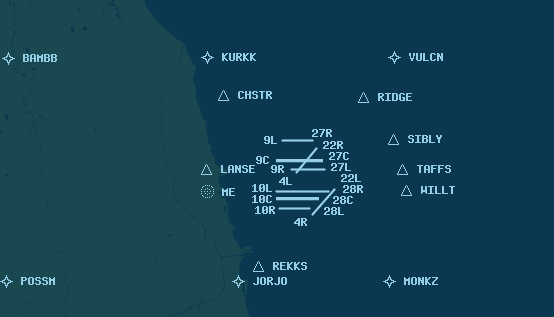
\includegraphics[width=0.75\textwidth]{existing_solutions/airportinseaatcsim.png}
\caption{\label{fig:airportinseaatcsim}Airport appears to be in the sea in ATC-SIM}
\end{figure}
\end{appendices}

\end{document}
